%main.tex
\documentclass[a4paper]{article}
%其余为默认值,需要的话再添加控制参数,详见《入门手册》

%——————————————————————导言区——————————————————————

\usepackage{float}
\usepackage{color}

%——————————————————————设置页眉页脚——————————————————————
\usepackage{fancyhdr}
%\usepackage{lastpage}%获得总页数

%——————————————————————设置摘要——————————————————————
\renewcommand{\abstractname}{摘要}

%——————————————————————设置目录样式——————————————————————
\usepackage{titlesec}  
\usepackage{titletoc}
\usepackage{xfrac}
\contentsmargin{0pt}\renewcommand\contentspage{\thecontentspage}
\renewcommand\contentsname{\centerline{目\hspace{1em}录}}%目录 二字居中
\dottedcontents{section}[0.66cm]{\addvspace{5pt}}{1em}{6pt}
%\dottedcontents{section}[0.66cm]{\addvspace{5pt}}{1em}{5pt}
\dottedcontents{subsection}[1.40cm]{}{1.7em}{5pt}
\dottedcontents{subsubsection}[2.51cm]{}{2.4em}{5pt}
%更改目录样式,addvspace更改了sec之间的行间距

%——————————————————————设置中文字体——————————————————————
\usepackage{xeCJK}
%\usepackage[no-config,quiet]{fontspec}%使用电脑自带字体
\setCJKmainfont[BoldFont ={SimHei},ItalicFont ={SimSun}]{SimSun}%设置中文正体字体,BoldFont设置粗体和斜体样式对应的字体
\setCJKsansfont{SimHei}%设置无衬线样式对应字体
\setCJKmonofont{SimSun}%设置有衬线样式对应字体
\punctstyle{hangmobanjiao} %行末半角式:所有标点占一个汉字宽度,行首行末对齐
\setCJKfamilyfont{hei}{SimHei}                        
\newcommand{\hei}{\CJKfamily{hei}} 
\newcommand{\con}{Consolas}

%——————————————————————设置字号——————————————————————
\newcommand{\xiaoerhao}{\fontsize{18pt}{\baselineskip}\selectfont}
\newcommand{\sihao}{\fontsize{14pt}{\baselineskip}\selectfont}
\newcommand{\wuhao}{\fontsize{10.5pt}{\baselineskip}\selectfont}
\newcommand{\xiaowuhao}{\fontsize{9pt}{\baselineskip}\selectfont}

%——————————————————————设置间距——————————————————————
\usepackage{setspace}%使用间距宏包
\setlength{\parskip}{0.2\baselineskip}%段间距 这个一般是0.5
%\renewcommand{\baselinestretch}{1}%行间距

%——————————————————————设置数学字体——————————————————————
%\usepackage{mathpazo,pxfonts}%配合数学字体palatino linotype使用的
\usepackage{times,amsmath,txfonts}%配合数学字体times new roman使用的
\usepackage{bm}
\let\iint\relax\let\iiint\relax\let\iiiint\relax\let\idotsint\relax\usepackage{amsmath}%解决冲突的
\newcommand*{\dif}{\mathop{}\!\mathrm{d}}%设置微分算子d

%——————————————————————设置英文字体——————————————————————
\setmainfont{Times New Roman}

%——————————————————————设置页边距————————————————————————
\usepackage{geometry}
\geometry{top=2.5cm, bottom=3cm, left=3.5cm, right=2.5cm}
\geometry{includehead,headheight=41pt}%设置页眉
\headrule{\addvspace{5pt}}

%——————————————添加首行缩进,两个字符—————————————————————
\usepackage{indentfirst}
\setlength{\parindent}{2em}
%\noindent %如果某段不缩进,段落开头用这个命令
%\indent   %如果某段要缩进,段落开头用这个命令

%————————————————————改善三线表粗细——————————————————————
\usepackage{booktabs}
\usepackage{longtable}
\usepackage{multirow} % 多行多列

\newcommand{\tabincell}[2]{
	\begin{tabular}{@{}#1@{}}#2\end{tabular}
}%s控制水平居中,也能实现表格内换行

\usepackage{array}%固定列宽可以使用 array 宏包的 p{2cm} 系列命令

\newcommand{\PreserveBackslash}[1]{\let\temp=\\#1\let\\=\temp}

\newcolumntype{C}[1]{>{\PreserveBackslash\centering}p{#1}}

\newcolumntype{R}[1]{>{\PreserveBackslash\raggedleft}p{#1}}

\newcolumntype{L}[1]{>{\PreserveBackslash\raggedright}p{#1}}
%使用C{3cm}命令即可指定该列宽度为3cm,并且文字居中对齐

%——————————————————————插入图片————————————————————————
\usepackage{graphicx}
%\includegraphics[width = .8\textwidth]{a.jpg}配套使用

%————————————————————章节居中——————————————————————
\usepackage{titlesec}

%————————————————————随章节号编号——————————————————————
\makeatletter
\@addtoreset{equation}{section}
\@addtoreset{figure}{section}
\@addtoreset{table}{section}
\makeatother%每个章节重新编号
\renewcommand{\theequation}{\thesection.\arabic{equation}}%公式编号中的那个是-连接,下面那个是.连接,如5-1
%\renewcommand{\theequation}{\thesection.\arabic{equation}}
\renewcommand{\thefigure}{\thesection.\arabic{figure}}
\renewcommand{\thetable}{\thesection.\arabic{table}}
\renewcommand{\figurename}{图}
\renewcommand{\tablename}{表}
\usepackage{cases}%多行公式编号需要

%————————————————————图\表格 标题居中——————————————————————
\usepackage[justification=centering]{caption}
\captionsetup[figure]{labelsep=space}%去掉图注的":"
\captionsetup[table]{labelsep=space}%去掉表注的":"

%————————————————————放置多张图片——————————————————————————
\usepackage{subfigure}
\usepackage{graphicx}
\usepackage{caption}
\usepackage{float}%图片浮动

%————————————————————调整caption的上下距离—————————————————
\setlength{\abovecaptionskip}{3pt}
\setlength{\belowcaptionskip}{-0pt}
\captionsetup{font={small}}%caption字号大小 footnotesize=小5号

%——————————————————————设置标题格式————————————————————————
\usepackage{titlesec}
\titleformat{\section}[block]{\sihao\hei\filcenter}{\thesection}{1em}{}
\titleformat{\subsection}{\wuhao\hei}{\thesubsection \hspace{0.68em}}{0em}{}
\titleformat{\subsubsection}{\wuhao\hei}{\hspace{2em}\thesubsubsection \hspace{0.68em}}{0em}{}

%——————————————————————参考文献————————————————————————
\usepackage{cite}
\renewcommand{\refname}{参考文献}
\newcommand{\upcite}[1]{\textsuperscript{\textsuperscript{\cite{#1}}}}%参考文献引用上标,用\upcite引用。

%——————————————————————附录————————————————————————
\usepackage{appendix}

%——————————————————————插入代码————————————————————————
\usepackage{listings}
\usepackage{xcolor} % 定制颜色
\definecolor{mygreen}{rgb}{0,0.6,0}
\definecolor{mygray}{rgb}{0.5,0.5,0.5}
\definecolor{mymauve}{rgb}{0.58,0,0.82}
\newfontfamily\con{Consolas}%设置代码字体

\begin{document}
	\pagestyle{fancy}
	\fancyhf{}  %全局设置,清空页眉页脚
	\lhead{
\includegraphics[scale=0.55]{fig/tongjilogo.png}}
	\rhead{机电液系统数字化建模与设计课程报告(一)}
	        
	%——————————————————————摘要——————————————————————
	%\include{data/Abstract} 否则会多一个空白页
	%\input{data/Abstract}
	
	%——————————————————————目录—————————————————————— 
	\tableofcontents
	%\contentsmargin{0pt}\renewcommand\contentspage{\thecontentspage}
	%\dottedcontents{section}[2.3em]{\bfseries\addvspace{10pt}}{2.3em}{5pt}
	%\dottedcontents{subsection}[5.5em]{}{3.2em}{5pt}
	%\thispagestyle{fancy}
	
	%—————————————————————章节部分—————————————————————
	\clearpage
\section{键合图优化}

\subsection{键合图因果划添加步骤}

\begin{itemize}
	\item 势源 $S_e$ 为势流出,所以因果划标在半箭头的外端;
	\item 势源 $S_f$ 为流流出,所以因果划标在半箭头的内端;
	\item 储能元件 $C I$ 先确定为积分因果关系,则 $C$ 元件的因果划标在半箭头的外端, $I$ 元件的因果划标在半箭头的内端;
	\item 0结为共势结,只能有一个流流出;
	\item 1结为共流结,只能有一个势流出;
	\item 结合 GY 和 TF 回转器和变换器的指定标法进行标注;
	\item 按照上面的原则对MPW和MDM的键合图标注因果划:
\end{itemize}

\subsection{MPW 系统键合图修改和简化}

\subsubsection{系统初步添加因果划}

据因果划的添加原则,对键合图初步添加因果划,如下图所示:
%%%%%%%%%%%%%%%%%
\begin{figure}[H]
	\centering
	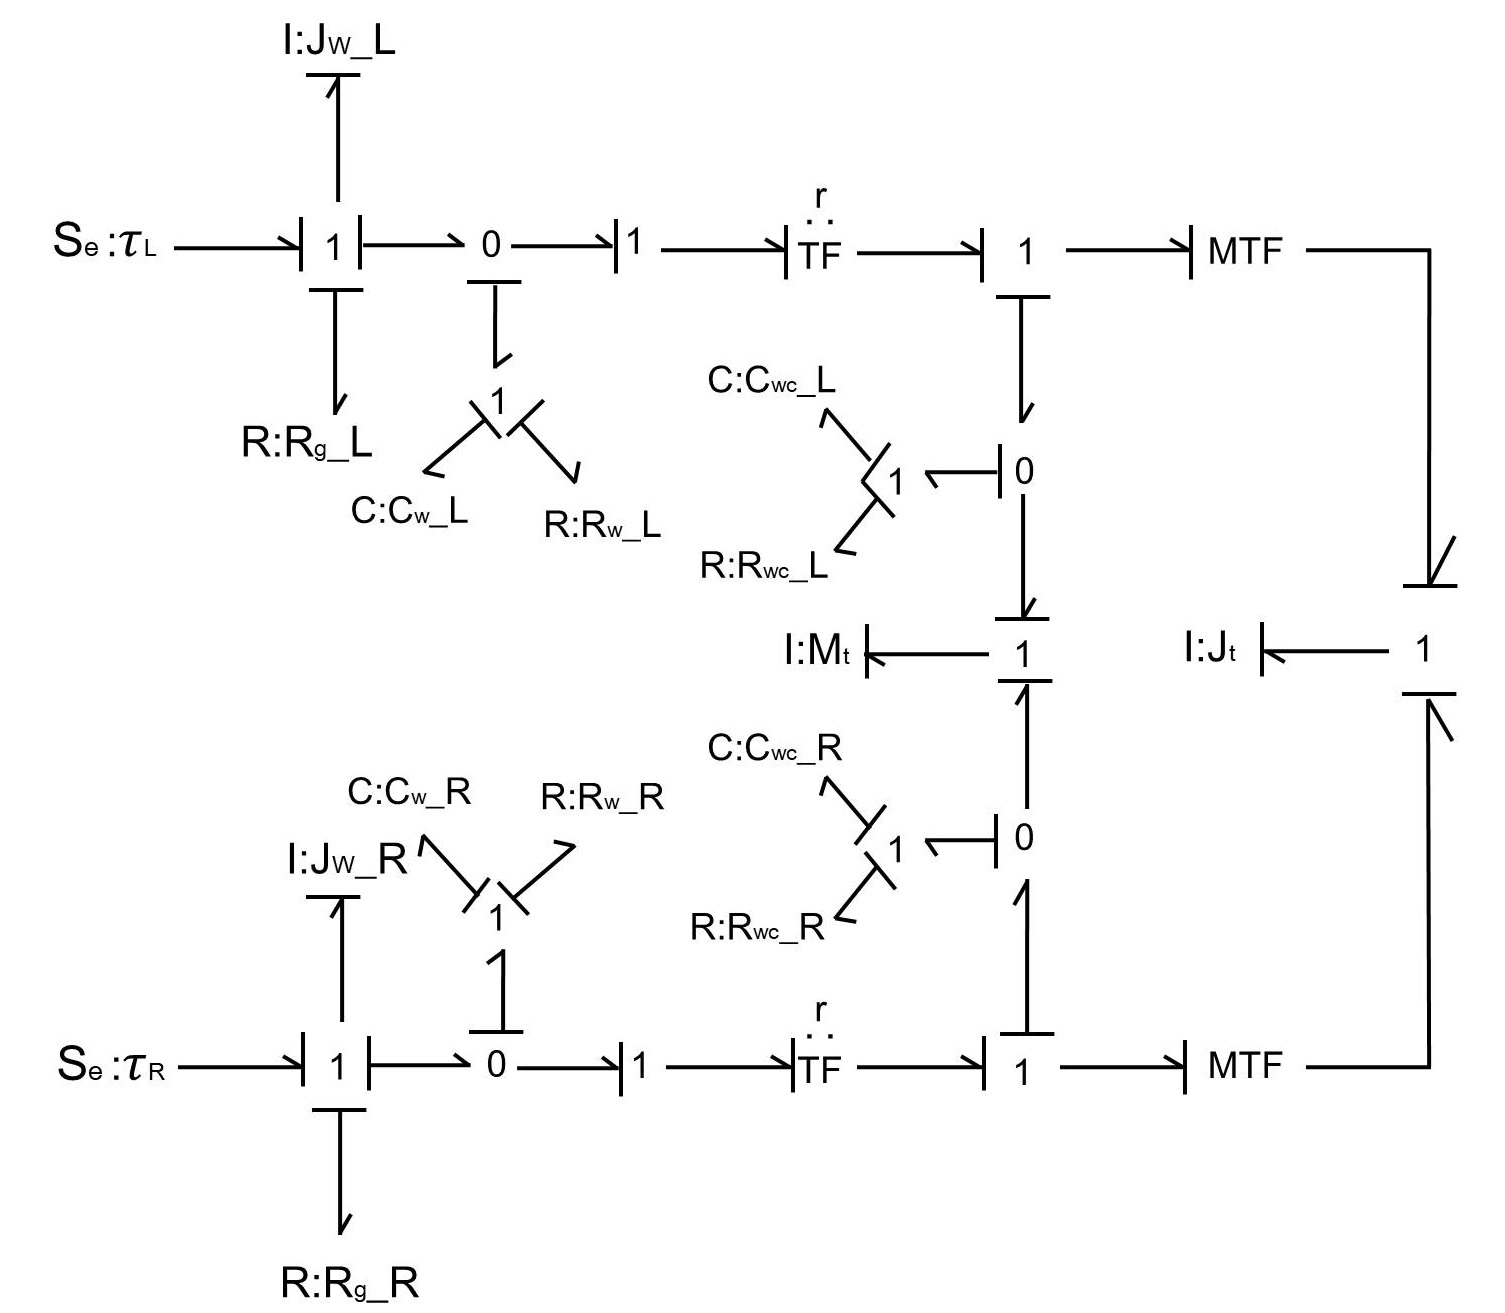
\includegraphics[width=0.6\textwidth]{fig/bond/MPW1.png}
	\caption{MPW系统因果划视图 }\label{fig:MPW1}
\end{figure}
%%%%%%%%%%%%%%%%%

\subsubsection{MPW系统键合图优化}

对于报告一中MPW模块的键合图,我们在此做了部分修改和优化,修改和优化后的部分如下图中红色方框中所示:
%%%%%%%%%%%%%%%%%
\begin{figure}[H]
	\centering
	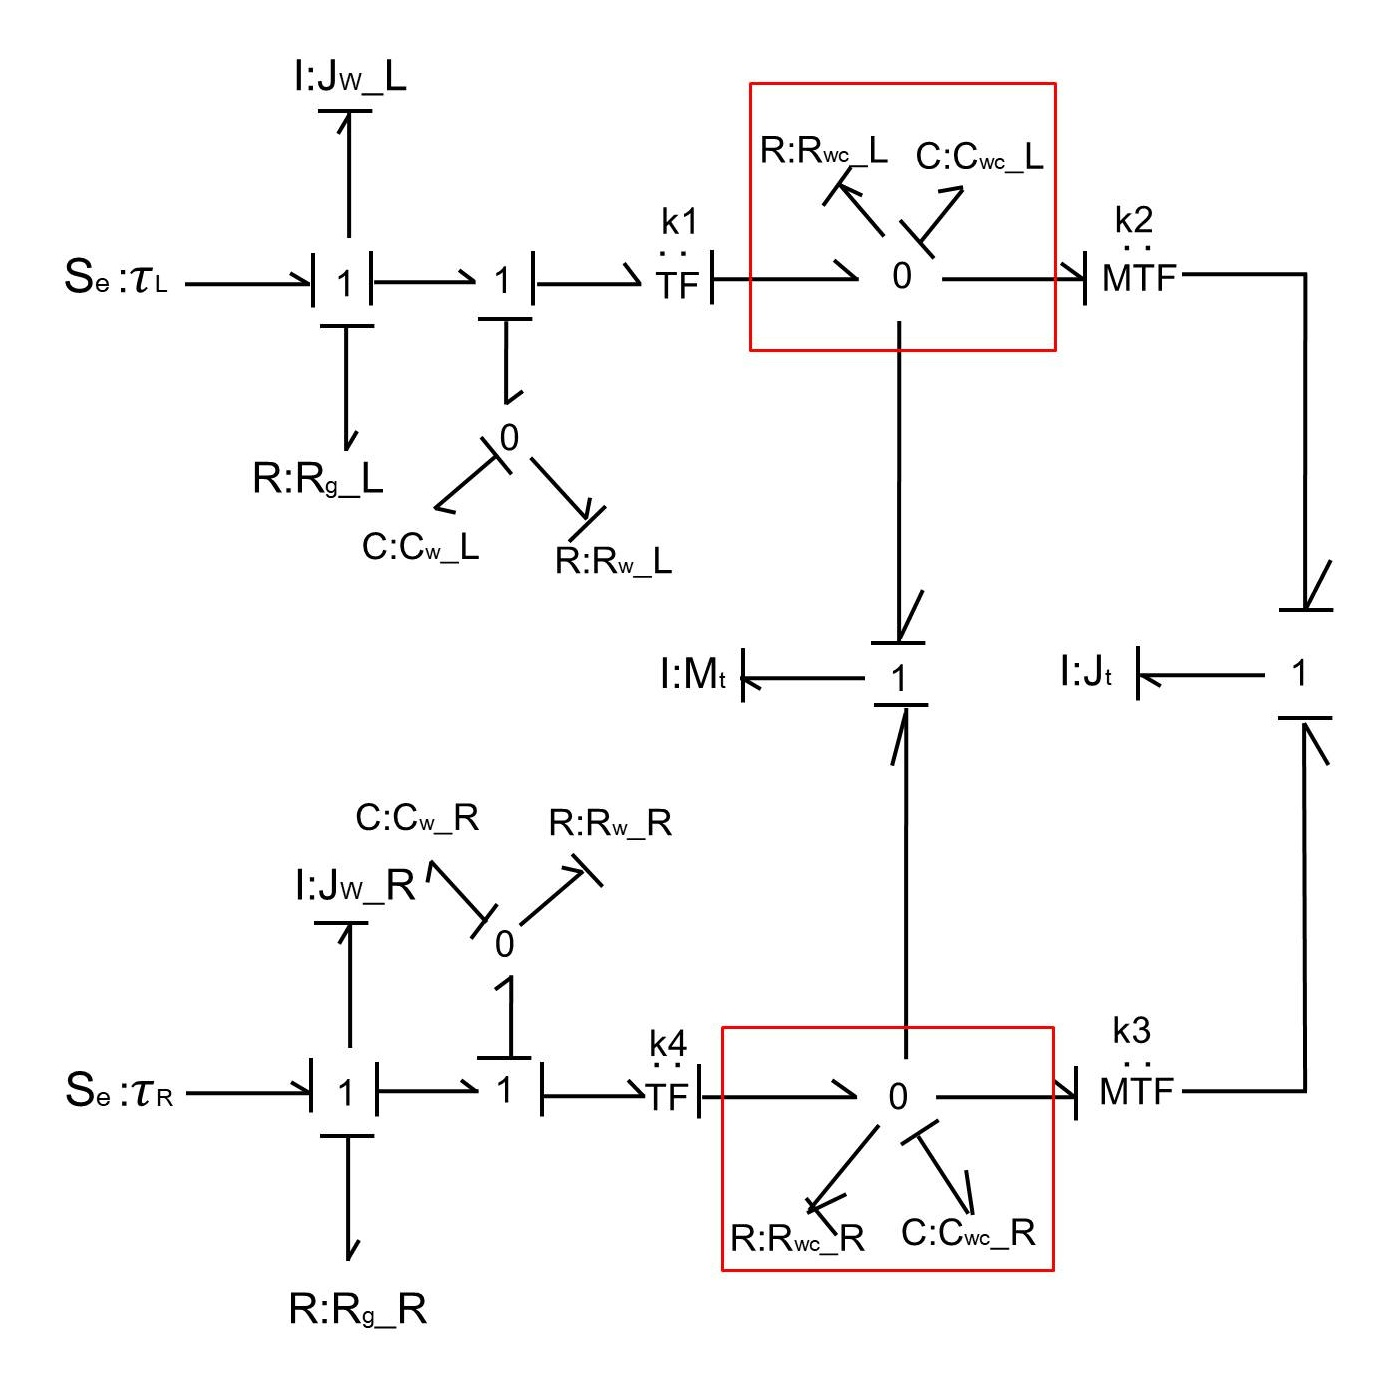
\includegraphics[width=0.6\textwidth]{fig/bond/MPW2.png}
	\caption{MPW系统优化键合图}\label{fig:MPW2}
\end{figure}
%%%%%%%%%%%%%%%%%

\subsection{MDM 系统键合图修改和简化}

\subsubsection{左轮电机模块简化与因果划添加}

根据因果划的添加原则,对电机模块的键合图初步添加因果划,如下图所示:
%%%%%%%%%%%%%%%%%
\begin{figure}[H]
	\centering
	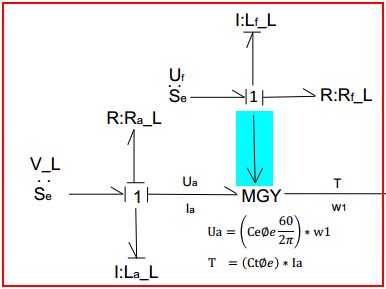
\includegraphics[width=0.5\textwidth]{fig/bond/MDM1.png}
	\caption{左轮电机模块因果划视图}\label{fig:bond_MDM1}
\end{figure}
%%%%%%%%%%%%%%%%%

对于他励直流电动机的驱动原理,电动机回路中电枢电压、电枢电流与电动机输出扭矩、输出角速度之间存在一个回转器的关系,如果励磁回路中的驱动磁场是变化的,则此回转器属于可变回转器MGY,励磁磁场直接影响的大小$ \Phi_e $,所以影响 $U_a=\left(C_e \Phi_e \frac{60}{2 \pi}\right) * w$ 和 $T=(C_t \Phi_e) * I_a$ 中的比例关系,属于可变回转器,为了简化实验,我们决定采用的是恒励磁磁场的模式,即励磁回路中的磁场恒定,所以此回转器属于定值回转器,并设定其系数为$ K_1 $,简化后的电机模块键合图如下图所示:
%%%%%%%%%%%%%%%%%
\begin{figure}[H]
	\centering
	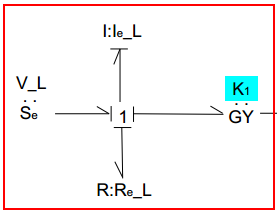
\includegraphics[width=0.5\textwidth]{fig/bond/MDM2.png}
	\caption{左轮电机模块简化键合图}\label{fig:bond_MDM2}
\end{figure}
%%%%%%%%%%%%%%%%%

同理可得右轮电机模块简化键合图。

\subsubsection{机械部分键合图简化与因果划添加}

根据因果划的添加原则,对MDM机械部分的键合图初步添加因果划,如下图所示:
%%%%%%%%%%%%%%%%%
\begin{figure}[H]
	\centering
	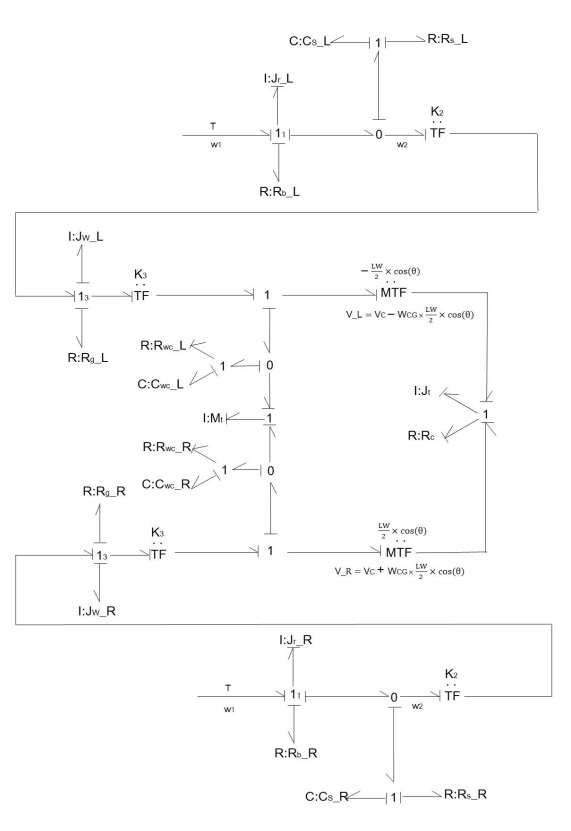
\includegraphics[width=0.55\textwidth]{fig/bond/MDM3.png}
	\caption{MDM机械部分因果划视图}\label{fig:bond_MDM3}
\end{figure}
%%%%%%%%%%%%%%%%%

为了方便仿真,我们对图进行来部分优化和修改优化,如下所示:
%%%%%%%%%%%%%%%%%
\begin{figure}[H]
	\centering
	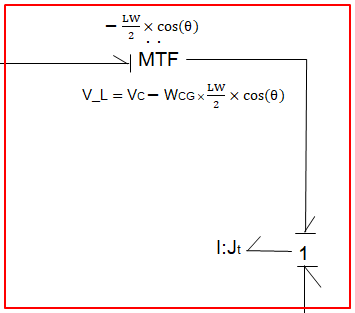
\includegraphics[width=0.5\textwidth]{fig/bond/MDM4.png}
	\caption{左轮变换器键合图}\label{fig:bond_MDM4}
\end{figure}
%%%%%%%%%%%%%%%%%

根据物理模型,左轮的线速度、整体模型的质心线速度、整体模型的质心角速度之间存在如下关系式:$v_L=v_C-w_{CG} \cdot \frac{L_w \cos(\theta)}{2}$ ,整体模型水平偏角 $ \theta $ 是变化的,所以此处存在一个可变变换器,为了方便仿真,我们决定采用寻找左右轮线速度瞬心的方法来确定变换器的系数,这种方法更加简便,这在后面章节中详细介绍,所以此处我们可以把变换器简化为下图所示,其中系数 $K_4$ 是变量:
%%%%%%%%%%%%%%%%%
\begin{figure}[H]
	\centering
	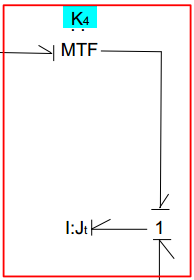
\includegraphics[width=0.35\textwidth]{fig/bond/MDM5.png}
	\caption{左轮变换器优化键合图}\label{fig:bond_MDM5}
\end{figure}
%%%%%%%%%%%%%%%%%

为了方便状态空间方程的建立,我们对报告一中的键合图两处进行了修改,修改后的键合图如下图所示,红色方框中为修改优化后的结果:
%%%%%%%%%%%%%%%%%
\begin{figure}[H]
	\centering
	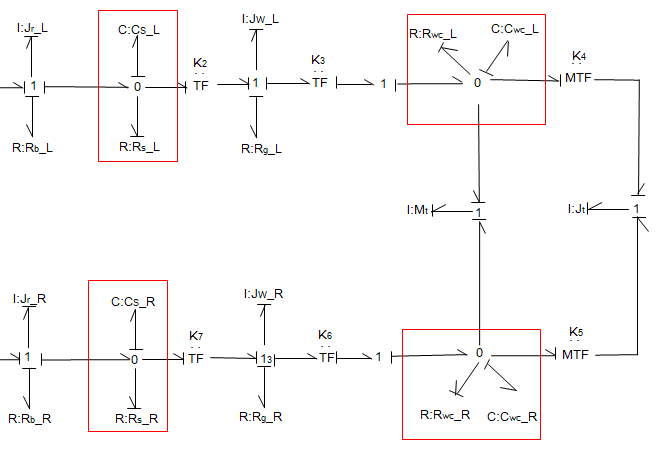
\includegraphics[width=0.8\textwidth]{fig/bond/MDM6.png}
	\caption{左轮变换器优化键合图}\label{fig:bond_MDM6}
\end{figure}
%%%%%%%%%%%%%%%%%

\subsubsection{MDM 模块的对接}

优化后的 MDM 总体键合图如下所示:
%%%%%%%%%%%%%%%%%
\begin{figure}[H]
	\centering
	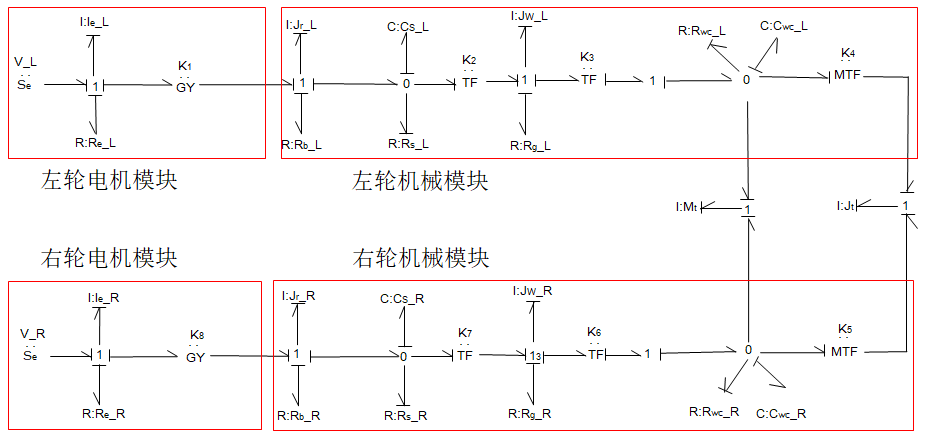
\includegraphics[width=0.8\textwidth]{fig/bond/MDM7.png}
	\caption{左轮变换器优化键合图}\label{fig:bond_MDM7}
\end{figure}
%%%%%%%%%%%%%%%%%

	\clearpage
\section{手推轮椅主体(Manual Propelled Wheelchair) 框图建模}

%%%%%%%%%%%%%%%%%
\begin{figure*}[h]
	\centering
	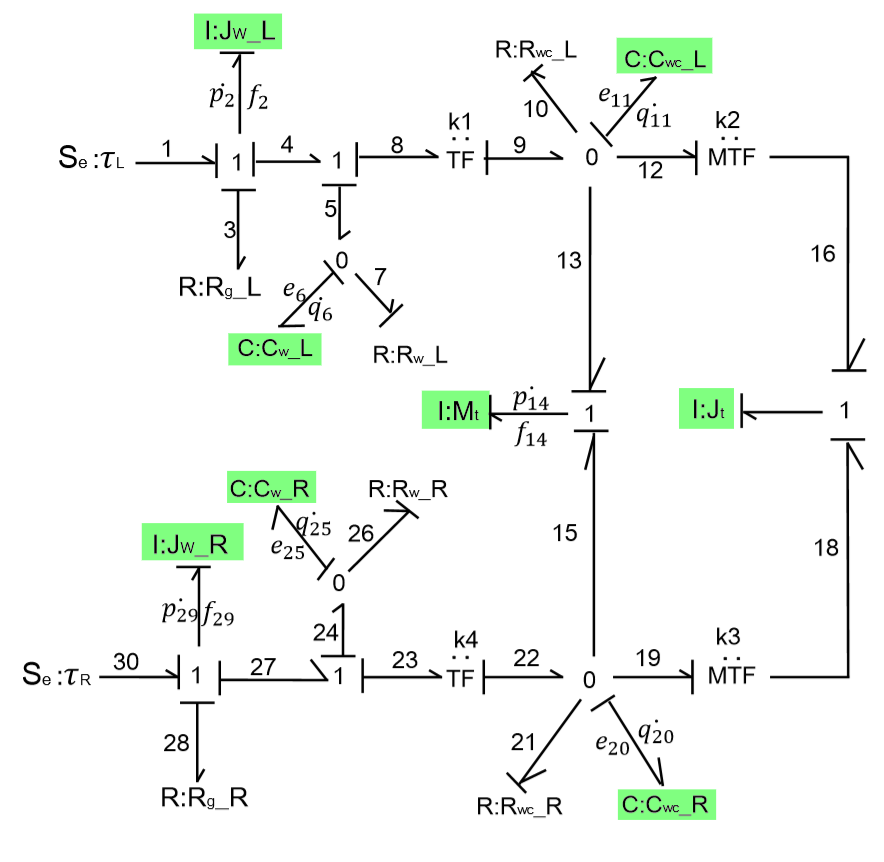
\includegraphics[width=0.7\textwidth]{fig/MPW.png}
	\caption{MPW因果化标注。}\label{fig:mdm}
\end{figure*}
%%%%%%%%%%%%%%%%%

\subsection{状态空间方程推导}

\begin{enumerate}

\item {后轮与地面运动状态变量$\dot{p}_2 $}

%%%%%%%%%%%%%%%%%
\begin{figure*}[h]
	\centering
	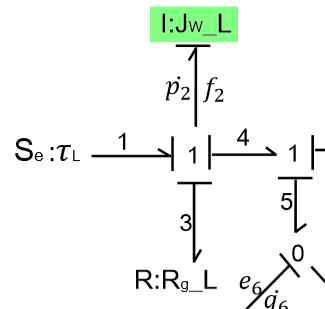
\includegraphics[width=0.4\textwidth]{fig/2_equation1.png}
\end{figure*}
%%%%%%%%%%%%%%%%%

对于$\dot{p} _ { 2 }$,开始列写方程,利用键合图的因果关系求出$e_2$:根据功率流方向标注,势变量$e_2$来自1结的输出,是由$e_1$,$e_3$,和$e_4$产生的,因此:

\begin{equation}\label{2_e2}
\dot{p}_{2}
=
e_2
=
e_1
-
e_3
-
e_4
=
\tau_L
-
e_3
-
e_4,
\end{equation}

$e_1$是输入变量,一直保留在最终的方程中;$e_3$来自阻性元件$R _ { eL }$的输出;$e_4$直接与状态变量有关,故而有下面三式:
\begin{equation}\label{2_e3}
e_3
=
f_3 \cdot R_{gL}
=
f_2 \cdot R_{gL}
=
\frac{p_{2}}{J_{wL}} R_{g L},
\end{equation}

\begin{equation}\label{2_e4}
e_4 = e_5 + e_8
=
e_6 + e_9 \cdot k_1
= 
\frac{q_{6}}{C_{wL}}
+
\frac{q_{11}}{C_{wcL}} k_{1},
\end{equation}

由式(\ref{2_e2})-(\ref{2_e4})得到状态方程1:
\begin{equation}\label{2_p2}
\dot{p}_{2}
=
\tau_{L}
-
\frac{p_{2}}{J_{wL}} R_{g L}
-
\frac{q_{11}}{C_{wcL}} k_{1}
-
\frac{q_{6}}{C_{wL}},
\end{equation}

%%%%%%%%%%%%%%%%%%%%%%%%%%%%%%%%%%%%%%%%%%%%%%%%%%%%%%%%%%%%%%%%
%%%%%%%%%%%%%%%%%%%%%%%%%%%%%%%%%%%%%%%%%%%%%%%%%%%%%%%%%%%%%%%%
%%%%%%%%%%%%%%%%%%%%%%%%%%%%%%%%%%%%%%%%%%%%%%%%%%%%%%%%%%%%%%%%
\item {后轮轮辐结构相关状态变量$\dot{q}_6 $}
%%%%%%%%%%%%%%%%%
\begin{figure}[H]
	\centering
	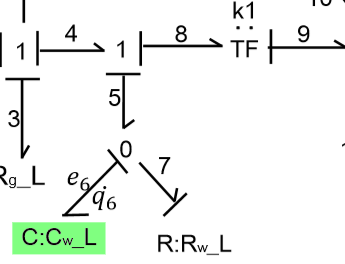
\includegraphics[width=0.4\textwidth]{fig/2_equation2.png}
\end{figure}
%%%%%%%%%%%%%%%%%
对于$\dot{q}_{ 6 }$,开始列写方程,利用键合图的因果关系求出$f_6$:根据功率流方向标注,流变量$f_6$来自0结的输出,是由$f_5$和$f_7$产生的,因此:
\begin{equation}\label{2_f6}
\dot{q}_{6}
=
f_6
=
f_5 - f_7,
\end{equation}
$f_5$直接与状态变量有关;$f_7$同样直接与状态变量有关,故而有下面两式:
\begin{equation}\label{2_f5}
f_5
=
f_4
=
f_2
=
\frac{p_{2}}{J_{w L}},
\end{equation}

\begin{equation}\label{2_f7}
f_7
=
\frac{e_{7}}{R_{w L}}
=
\frac{e_{6}}{R_{w L}}
=
\frac{q_{6}}{C_{wL} R_{w L}},
\end{equation}

由式(\ref{2_f6})-(\ref{2_f7})得到状态方程2:
\begin{equation}\label{2_q6}
\dot{q}_{6}
=
\frac{p_{2}}{J_{w L}}-\frac{q_{6}}{C_{wL} R_{w L}}.
\end{equation}

%%%%%%%%%%%%%%%%%%%%%%%%%%%%%%%%%%%%%%%%%%%%%%%%%%%%%%%%%%%%%%%%
%%%%%%%%%%%%%%%%%%%%%%%%%%%%%%%%%%%%%%%%%%%%%%%%%%%%%%%%%%%%%%%%
%%%%%%%%%%%%%%%%%%%%%%%%%%%%%%%%%%%%%%%%%%%%%%%%%%%%%%%%%%%%%%%%
\item {后轮与整体解耦相关状态变量$\dot{q}_{11}$}
%%%%%%%%%%%%%%%%%
\begin{figure*}[h]
	\centering
	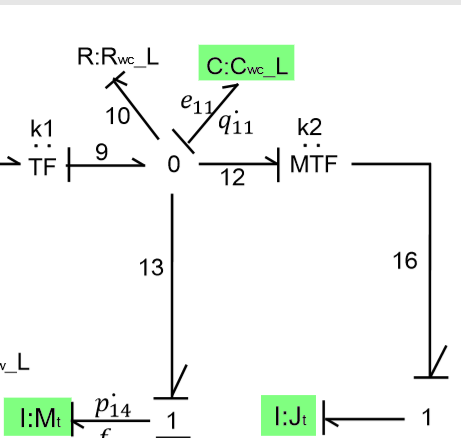
\includegraphics[width=0.4\textwidth]{fig/2_equation3.png}
\end{figure*}
%%%%%%%%%%%%%%%%%
对于$\dot{q} _ { 11 }$,
开始列写方程,通过使用因果关系对$f_11$路径进行跟踪,流变量$f_11$是对$C_{wcL}$的输入,从0结出来的输出,此输出由因果输入$f _ { 9 }$, $ f _ { 10 }$, $  f _ { 12 }$和$f _ { 13 }$产生,因此:
\begin{equation}\label{2_f11}
\dot{q}_{11}
=
f_{11}
=
f_9 - f_{10} - f_{12} - f_{13},
\end{equation}
$f_9$来自TF元件;$f_{10}$来自阻性元件$R _ { wcL }$的输出;$f_{12}$和$f_{13}$同样直接与状态变量有关,故而有下面四式:
\begin{equation}\label{2_f9}
f_{9}
=
f_{8} \cdot k_1
=
f_{4} \cdot k_1
=
f_{2} \cdot k_1
=
\frac{p_{2}}{J_{w L}} k_{1},
\end{equation}

\begin{equation}\label{2_f10}
f_{10}
=
\frac{e_{10}}{R_{wc L}}
=
\frac{e_{11}}{R_{wc L}}
=
\frac{q_{11}}{C_{wc L} R_{wc L}},
\end{equation}

\begin{equation}\label{2_f12}
f_{12}
=
\frac{f_{16}}{k_{2}} 
=
\frac{f_{17}}{k_{2}} 
=
\frac{p_{17}}{J_{t} k_{2}},
\end{equation}

\begin{equation}\label{2_f13}
f_{13}
=
f_{14}
=
\frac{p_{14}}{M_{t}},
\end{equation}

由式\ref{2_f11}-\ref{2_f13}得到状态方程3:
\begin{equation}\label{2_q11}
\dot{q}_{11}
=
\frac{p_{2}}{J_{w L}} k_{1}
-
\frac{q_{11}}{C_{wc L} R_{wc L}}
-
\frac{p_{17}}{J_{t} k_{2}}
-
\frac{p_{14}}{M_{t}}.
\end{equation}

%%%%%%%%%%%%%%%%%%%%%%%%%%%%%%%%%%%%%%%%%%%%%%%%%%%%%%%%%%%%%%%%
%%%%%%%%%%%%%%%%%%%%%%%%%%%%%%%%%%%%%%%%%%%%%%%%%%%%%%%%%%%%%%%%
%%%%%%%%%%%%%%%%%%%%%%%%%%%%%%%%%%%%%%%%%%%%%%%%%%%%%%%%%%%%%%%%
\item {质心处状态分析(质量)状态变量$\dot{ p}_{14} $}
%%%%%%%%%%%%%%%%%
\begin{figure}[H]
	\centering
	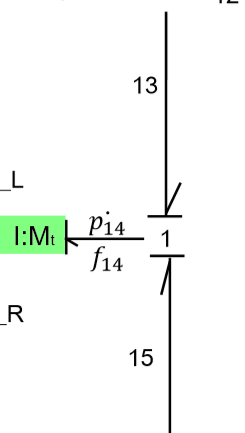
\includegraphics[width=0.25\textwidth]{fig/2_equation4.png}
\end{figure}
%%%%%%%%%%%%%%%%%
对于$\dot{p} _ { 14 }$,开始列写方程,利用键合图的因果关系求出$e_{14}$:根据功率流方向标注,势变量$e_{14}$来自1结的输出,是由$e_{13}$和$e_{15}$产生的,因此:
\begin{equation}\label{2_e14}
\dot{p}_{14}
=
e_{14}
=
e_{13}
+
e_{15},
\end{equation}
$e_{13}$和$e_{15}$均来自容性元件$C _ { wc }$的输出故而有下面两式:
\begin{equation}\label{2_e13}
e_{13}
=
e_{11}
=
\frac{q_{11}}{C_{wc L}},
\end{equation}

\begin{equation}\label{2_e15}
e_{15}
=
e_{20}
=
\frac{q_{20}}{C_{wc R}},
\end{equation}

由式\ref{p13}-\ref{e15}得到状态方程4:
\begin{equation}\label{2_p14}
\dot{p}_{14}
=
\frac{q_{11}}{C_{wc L}}
+
\frac{q_{20}}{C_{wc R}}.
\end{equation}

%%%%%%%%%%%%%%%%%%%%%%%%%%%%%%%%%%%%%%%%%%%%%%%%%%%%%%%%%%%%%%%%
%%%%%%%%%%%%%%%%%%%%%%%%%%%%%%%%%%%%%%%%%%%%%%%%%%%%%%%%%%%%%%%%
%%%%%%%%%%%%%%%%%%%%%%%%%%%%%%%%%%%%%%%%%%%%%%%%%%%%%%%%%%%%%%%%
\item {质心处状态分析(转动惯量)状态变量$\dot{ p}_{17}$}
%%%%%%%%%%%%%%%%%
\begin{figure*}[h]
	\centering
	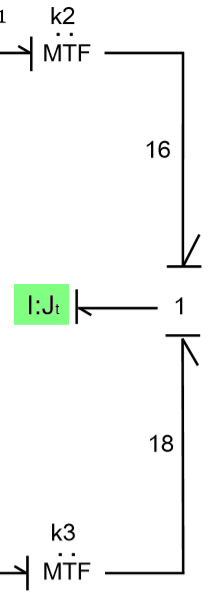
\includegraphics[width=0.25\textwidth]{fig/2_equation5.png}
\end{figure*}
%%%%%%%%%%%%%%%%%
对于$\dot{p} _ { 17 }$,开始列写方程,通过使用因果关系对$p_{17}$路径进行跟踪,从1结出来的输出,此输出由因果输入$e _ { 16 }$和$  e _ { 18 }$产生,因此:
\begin{equation}\label{2_p17}
\dot{p}_{17}
=
e_{17}
=
e_{16}
+
e_{18},
\end{equation}

$e _ { 16 }$和$e_{18}$来自MTF元件的输入,故而有下面两式:
\begin{equation}\label{2_e16}
e_{16}
=
\frac{e_{12}}{k_2}
=
\frac{e_{11}}{k_2}
=
\frac{q_{11}}{C_{w L} k_{3}},
\end{equation}

\begin{equation}\label{2_e18}
e_{18}
=
\frac{e_{19}}{k_3}
=
\frac{e_{20}}{k_3}
=
\frac{q_{20}}{C_{wc R}},
\end{equation}

由式\ref{2_p17}-\ref{2_e18}得到状态方程5:
\begin{equation}
\dot{p}_{17}
=
\frac{q_{11}}{C_{w L} k_{3}}
+
\frac{q_{20}}{k_{2} C_{w R}}.
\end{equation}

%%%%%%%%%%%%%%%%%%%%%%%%%%%%%%%%%%%%%%%%%%%%%%%%%%%%%%%%%%%%%%%%
%%%%%%%%%%%%%%%%%%%%%%%%%%%%%%%%%%%%%%%%%%%%%%%%%%%%%%%%%%%%%%%%
%%%%%%%%%%%%%%%%%%%%%%%%%%%%%%%%%%%%%%%%%%%%%%%%%%%%%%%%%%%%%%%%
\item {根据对称性得到剩余状态方程}
根据对称性,另外三个状态方程可以推出(\ref{2_q20})-(\ref{2_q29}):
\begin{equation}\label{2_q20}
\dot{q}_{20}
=
\frac{p_{29}}{J_{w R}} k_{1}
-
\frac{p_{14}}{M_{t}}
-
\frac{p_{17}}{J_{t} k_{3}}
-
\frac{q_{20}}{R_{wc R} C_{wc R} },
\end{equation}

\begin{equation}\label{2_q25}
\dot{q}_{25}=\frac{p_{29}}{J_{w_{-} R}}-\frac{q_{25}}{R_{w_{-} R} C_{w_{-}} R},
\end{equation}

\begin{equation}\label{2_q29}
\dot{p}_{29}
=
\tau_{R}-\frac{p_{29}}{J_{w R}} R_{g R}
-
\frac{q_{20}}{C_{wc R}} k_{1}
-
\frac{q_{25}}{C_{w R}}.
\end{equation}

\end{enumerate}

\subsection{总体状态空间矩阵}

\subsubsection{状态空间矩阵导出}

下列公式显示了MPW的状态空间表示,其中$ x_1$,$u_1$和$y_1$分别是系统状态,输入和输出:

\begin{equation}\label{2_dot_x1}
\dot{x}_1 =[\mathbf{A}_1] x_1+[\mathbf{B}_1] u_1,
\end{equation}

\begin{equation}\label{2_y1}
y_1 =[\mathbf{C}_1] x_1.
\end{equation}

由上述八个状态空间方程(\ref{2_p2}) ~ (\ref{2_q29}),具体表示成:

\begin{equation}\label{2_matrix1}
\begin{aligned}
\left[ 
\begin{array}
{l}{e_{2}} \\ {f_{6}} \\ {f_{11}} \\ {e_{14}} \\ {e_{17}} \\ {f_{20}} \\ {f_{25}} \\ {e_{25}}
\end{array}
\right] 
=
\left[ 
\begin{array}
{c}{\dot{p}_{2}} \\ {\dot{q}_{6}} \\ {\dot{q}_{11}} \\ {\dot{p}_{14}} \\ {\dot{p}_{17}} \\ {\dot{q}_{20}} \\ {\dot{q}_{25}} \\ {\dot{p}_{29}}
\end{array}
\right]
=
&
\left[ 
\begin{array}{cccccccc}
{- \frac{R_{gL}}{J_{w L}}} & - \frac{1}{C_{wL}} & - \frac{k_1}{C_{w L}} & 0 & 0 & 0 & 0 & 0 \\ 
\frac{1}{J_{w L}} & - \frac{1}{R_{wL} C_{wL}} & 0 & 0 & 0 & 0 & 0 & 0 \\ 
\frac{k_{1}}{J_{W_L}}  & 0 & - \frac{1}{R_{wc L} C_{wc L}} & - \frac{1}{M_{t}} & - \frac{1}{k_{2} J_{t}} & 0 & 0 & 0  \\ 
0 & 0 & \frac{1}{C_{wc L}} & 0 & 0 & \frac{1}{C_{wc R}}  & 0 & 0   \\ 
0 & 0 & \frac{1}{k_{3} C_{wc L}} & 0 & 0 & \frac{1}{k_{2} C_{wc R}}  & 0 & 0  \\ 
0 & 0 & 0 & - \frac{1}{M_{t}} & - \frac{1}{k_{2} J_{t}} & - \frac{1}{R_{wc R} C_{wc R}} & 0 & \frac{k_{1}}{J_{W_R}} \\ 
0 & 0 & 0 & 0 & 0 & 0 & - \frac{1}{R_{w R}  C_{w R}} & \frac{1}{J_{w R}}  \\ 
0 & 0 & 0 & 0 & 0 & - \frac{k_{1}}{C_{wc R}} & - \frac{1}{C_{w R}} &  - \frac{R_{g R}}{J_{wR}} 
\end{array}
\right]
\left[
\begin{array}{c}
{p_{2}} \\ {q_{6}} \\ {q_{11}} \\ {p_{14}} \\ {p_{17}} \\ {q_{20}} \\ {q_{25}} \\ {q_{29}}
\end{array}
\right]
\\
&+
\left[ 
\begin{array}{ll}
{1} & {0} \\ {0} & {0} \\ {0} & {0} \\ {0} & {0} \\ {0} & {0} \\ {0} & {0} \\ {0} & {0} \\ {0} & {1}
\end{array}
\right]
\left[ \begin{array}{l}
{\tau_{L}} \\ {\tau_{R}}
\end{array}\right]
\end{aligned}.
\end{equation}

则输出矩阵则表示为:

\begin{equation}\label{2_matrix2}
\left[
\begin{array}{c}{\omega_{L}} \\ {\omega_{R}} \\ {V_{C G}} \\ {\theta_{C G}}
\end{array}
\right]
=
\left[
\begin{array}{c}{f_{2}} \\ {f_{29}} \\ {f_{14}} \\ {f_{17}}\end{array}
\right]
=
\left[ \begin{array}{cccc}
{\frac{1}{J_{w L}}} & {0} & {0} & {0} \\ {0} & {\frac{1}{J_{w R}}} & {0} & {0} \\ {0} & {0} & {\frac{1}{M_{t}}} & {0} \\ {0} & {0} & {0} & {\frac{1}{J_{t}}}
\end{array}\right] 
\left[ \begin{array}{c}
{p_{2}} \\ {p_{29}} \\ {p_{17}} \\ {p_{17}}
\end{array}\right].
\end{equation}

\subsubsection{特殊变量分析}

特别地,其中的$ k_2 $ 和 $ k_3 $ 属于根据速度变化的动态变量,分别代表转动过程中左右轮相对速度瞬心的曲率半径,需要根据两轮机器人模型导出:

%%%%%%%%%%%%%%%%%
\begin{figure*}[!b]
	\centering
	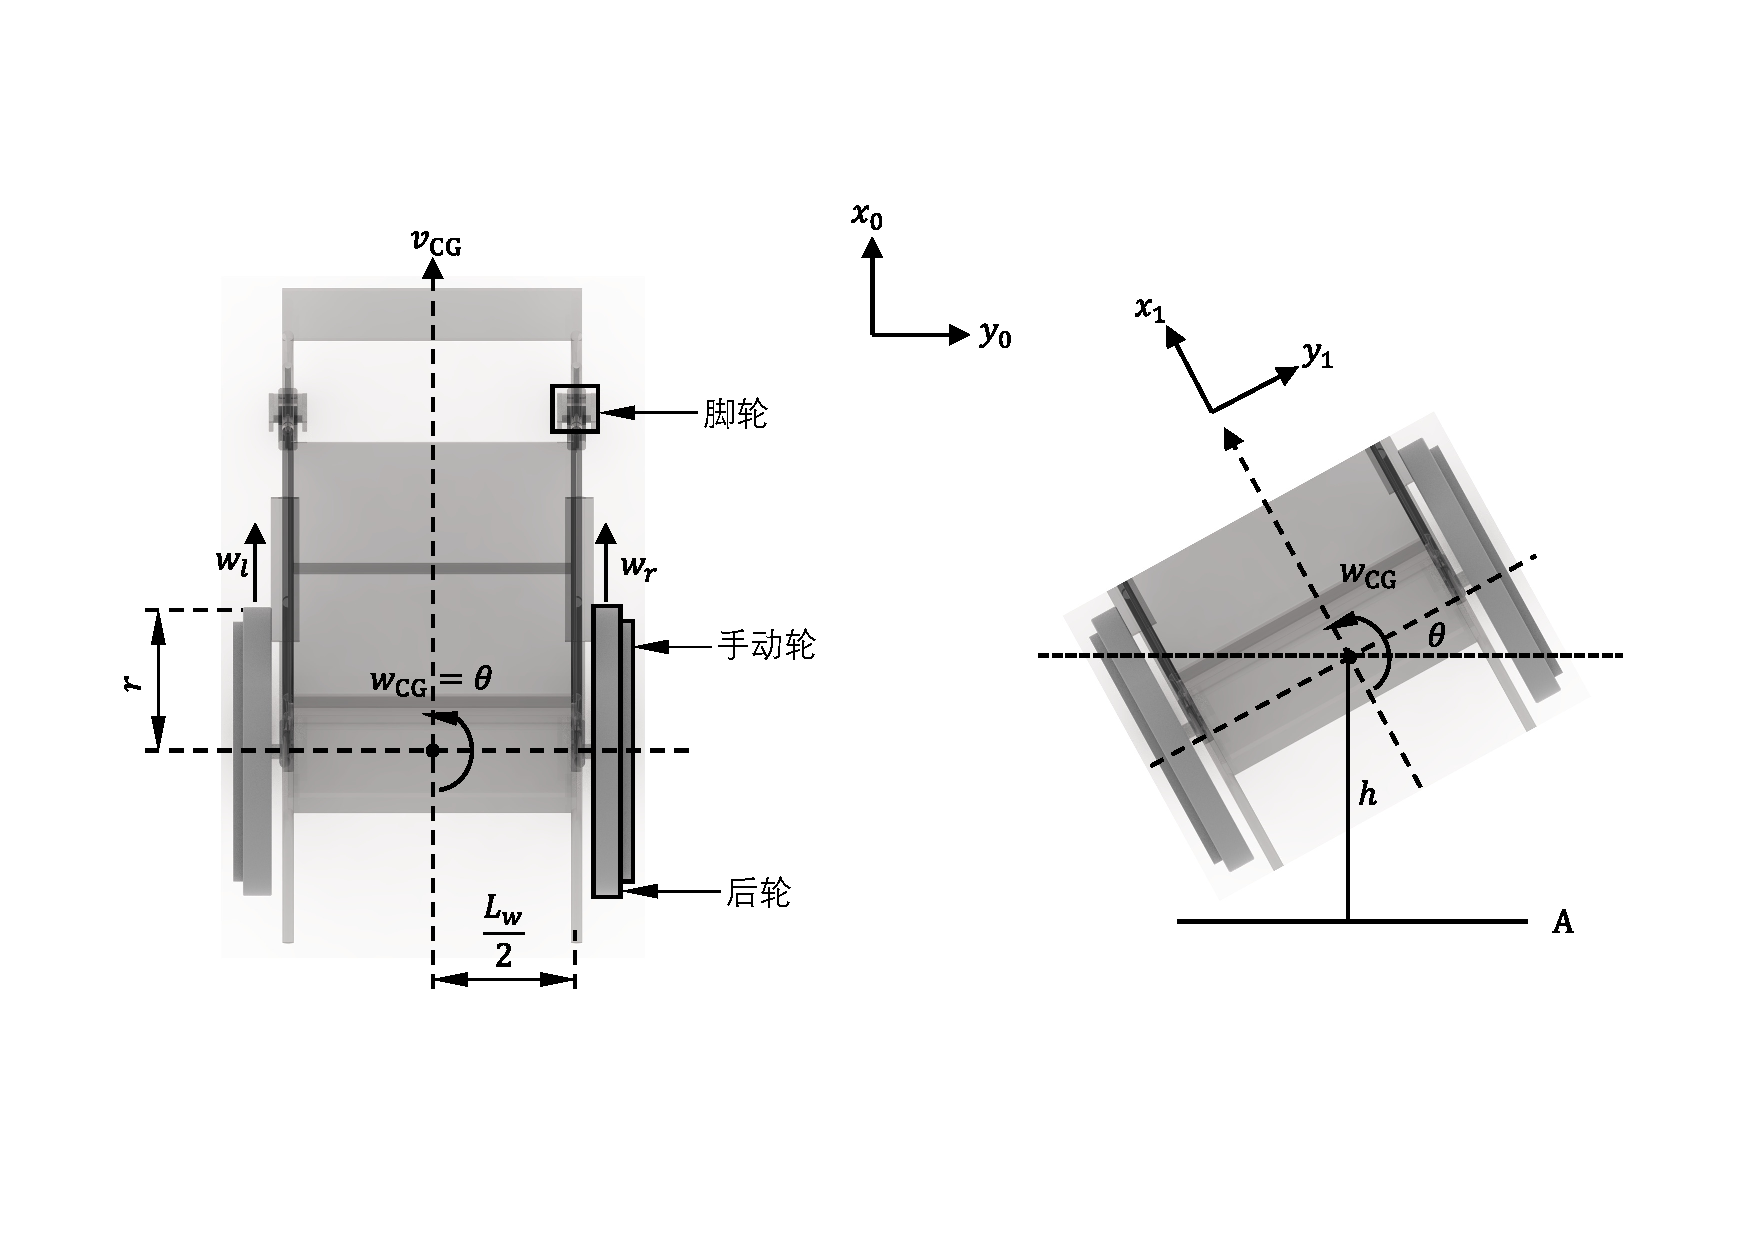
\includegraphics[width=0.95\textwidth]{fig/top_view.pdf}
	\caption{电动轮椅主体俯视示意图。}\label{fig:top_view}
\end{figure*}
%%%%%%%%%%%%%%%%%

在该建模中选取对象的机械主体示意如图 \ref{fig:top_view} 所示。它基本上由两个脚轮和手动后轮组成。在这种建模中已经应用了两轮驱动机器人系统的方法,其中脚轮集中在一起并且假设对系统流施力。 
$ V_{\rm{CG}} $ 和 $ w_{\rm{CG}} $ 代表质心速度和沿质心转速,$ w_l $ 和 $ w_r $ 分别表示左右车轮的角速度,后手动车轮半径和轮椅宽度由 $ r $ 和 $ L_w $ 表示)。
下面的矩阵\ref{equ:basic_eq}显示了系统的运动学数学模型,其中 $ \theta $ 是方位角,$ x $ 和 $ y $ 分别表示系统的几何位置:

%%%%%%%%%%%%%%%%%%%%%%%%%%
\begin{equation}
\label{equ:basic_eq}
\begin{bmatrix} \begin{array}{l}{x} \\ {y} \\ {\theta}\end{array} \end{bmatrix}
=
r
\begin{bmatrix}
\vspace{0.2cm} {\dfrac{\cos \theta}{2}} & {\dfrac{\cos \theta}{2}} \\
\vspace{0.2cm} {\dfrac{2}{L}} & {\dfrac{\sin \theta}{2}} \\
{\dfrac{2}{L_w}} & - {\dfrac{2}{L_w}}
\end{bmatrix}
\begin{bmatrix} \begin{array}{c}{\omega_r} \\ {\omega_l}\end{array} \end{bmatrix}
\ .
\end{equation}
%%%%%%%%%%%%%%%%%%%%%%%%%%

以A作为参考点,左右轮的位移课以得到: 

%%%%%%%%%%%%%%%%%%%%%%%%%%
\begin{equation}
\label{equ:left_s}
S_l = h
-
\frac{L_w}{2} \sin \theta
\ ,
\end{equation}
%%%%%%%%%%%%%%%%%%%%%%%%%%

%%%%%%%%%%%%%%%%%%%%%%%%%%
\begin{equation}
\label{equ:right_s}
S_r = h
+
\frac{L_w}{2} \sin \theta
\ .
\end{equation}
%%%%%%%%%%%%%%%%%%%%%%%%%%

从键合图出发,广义位移变量定义为流变量的时间积分。因此根据上述方程 \ref{equ:left_s} 和 \ref{equ:right_s},可以获得了所需的流变量方程,将可以通过方程 \ref{equ:left_s} 和 \ref{equ:right_s} 用于构建轮椅主体结构的键合图模型。

%%%%%%%%%%%%%%%%%%%%%%%%%%
\begin{equation}
\label{equ:left_v}
v_{l}
=
\dot{S}_{l}
=
\dot{h}
-
\dot{\theta} \frac{L_w}{2} \cos \theta
\ ,
\end{equation}
%%%%%%%%%%%%%%%%%%%%%%%%%%

%%%%%%%%%%%%%%%%%%%%%%%%%%
\begin{equation}
\label{equ:right_v}
v_{r}
=
\dot{S}_{r}
=
\dot{h}
+
\dot{\theta} \frac{L_w}{2} \cos \theta
\ .
\end{equation}
%%%%%%%%%%%%%%%%%%%%%%%%%%

进一步,假设此时$ v_{r} > v_{l} $,则 $ k_3 > k_2 $。根据瞬心的相关几何关系,我们可以得到下列式子:

%%%%%%%%%%%%%%%%%%%%%%%%%%
\begin{equation}\label{equ:k2k3_equs}
\frac{v_L}{k_2} = \frac{v_R}{k_3}.
\end{equation}
%%%%%%%%%%%%%%%%%%%%%%%%%%

其中,由假设与集合关系可得:

%%%%%%%%%%%%%%%%%%%%%%%%%%
\begin{equation}\label{equ:k2k3_Lw}
k_3 = k_2 + L_w.
\end{equation}
%%%%%%%%%%%%%%%%%%%%%%%%%%

结合上述两式可以导出:

%%%%%%%%%%%%%%%%%%%%%%%%%%
\begin{equation}\label{equ:k2_solution}
k_2 = \frac{v_L \times L_w}{v_R - v_L}.
\end{equation}
%%%%%%%%%%%%%%%%%%%%%%%%%%

为了方便编程与建模,上面方程 \ref{equ:k2_solution} 可以写成更一般的形式:

%%%%%%%%%%%%%%%%%%%%%%%%%%
\begin{equation}\label{equ:k2k3}
\begin{aligned}
\min (k_2, k_3) &= \frac{\min (v_L, v_R) \times L_w}{|v_R - v_L|} \\
\max (k_2, k_3) &= \frac{\max (v_L, v_R) \times L_w}{|v_R - v_L|}
\end{aligned}
\end{equation}
%%%%%%%%%%%%%%%%%%%%%%%%%%

	\clearpage
\section{电动轮椅(Mmechatronic drive module) 框图建模}

%%%%%%%%%%%%%%%%%
\begin{figure*}[h]
	\centering
	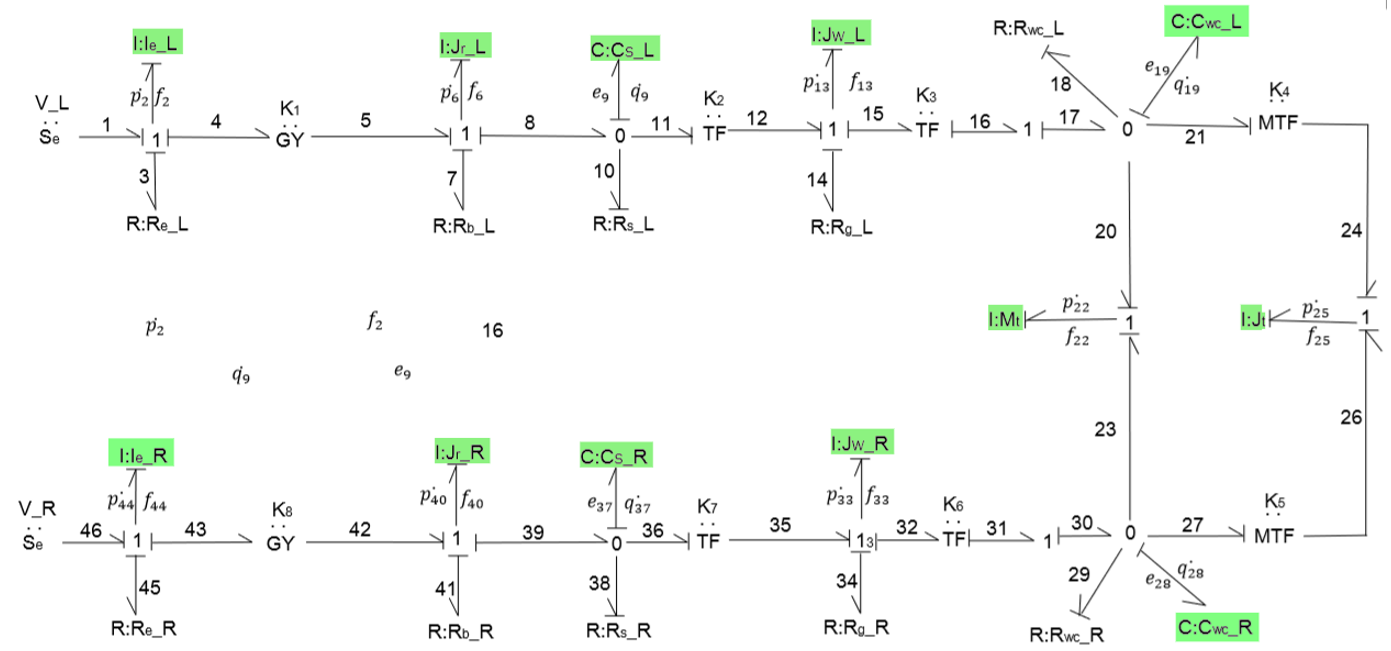
\includegraphics[width=\textwidth]{fig/MDM.png}
	\caption{MDM因果化标注。}\label{fig:mdm}
\end{figure*}
%%%%%%%%%%%%%%%%%
\subsection{状态空间方程推导}

\begin{enumerate}

\item {电机电特性状态变量$\dot{ p_2 }$}
%%%%%%%%%%%%%%%%%
\begin{figure*}[h]
	\centering
	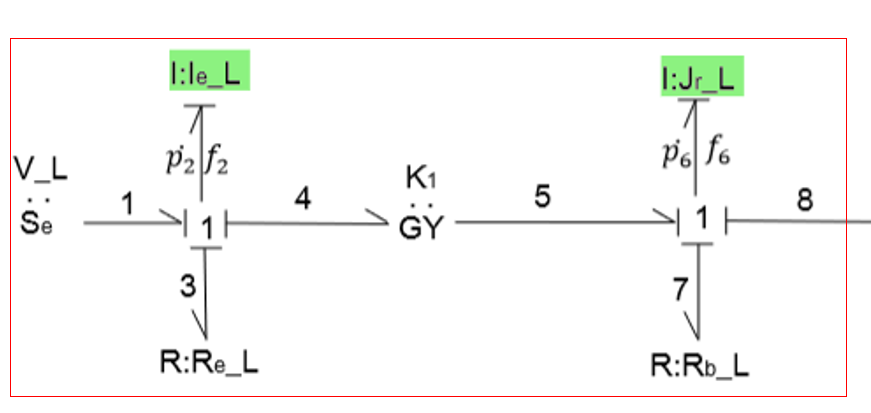
\includegraphics[width=0.5\textwidth]{fig/equation1.png}
	\caption{}\label{fig:equation1}
\end{figure*}
%%%%%%%%%%%%%%%%%
对于$\dot{p} _ { 2 }$,开始列写方程,利用键合图的因果关系求出$e_2$:根据功率流方向标注,势变量$e_2$来自1结的输出,是由$e_1$,$e_3$,和$e_4$产生的,因此:
\begin{equation}\label{p2}
\dot{p} _ { 2 } = e _ { 2 } = e _ { 1 } - e _ { 3 } - e _ { 4 },
\end{equation}
$e_1$是输入变量,一直保留在最终的方程中;$e_3$来自阻性元件$R _ { eL }$的输出;$e_4$直接与状态变量有关,故而有下面三式:
\begin{equation}\label{e1}
e _ { 1} = V_L,
\end{equation}

\begin{equation}\label{e3}
e _ { 3 } = f _ { 3 } R _ { eL  }  = f _ { 2 } R _ { eL }  = \frac { p _ { 2 } } { I _ { eL } } R _ { eL},
\end{equation}

\begin{equation}\label{e4}
e _ { 4 } = k _ { 1 } f _ { 5 } = k _ { 1 } f _ { 6 } = k _ { 1 } \frac { p _ { 6 } } { J _ { r L}  },
\end{equation}

由式(\ref{p2})-(\ref{e4})得到状态方程1:
\begin{equation}
\dot { p } _ { 2 } = V _ {L}  - \frac { p _ { 2 } } { I _ { eL}  } R _ { eL} - k _ { 1 } \frac { p _ { 6 } } { J _ { rL} },
\end{equation}

%%%%%%%%%%%%%%%%%%%%%%%%%%%%%%%%%%%%%%%%%%%%%%%%%%%%%%%%%%%%%%%%
%%%%%%%%%%%%%%%%%%%%%%%%%%%%%%%%%%%%%%%%%%%%%%%%%%%%%%%%%%%%%%%%
%%%%%%%%%%%%%%%%%%%%%%%%%%%%%%%%%%%%%%%%%%%%%%%%%%%%%%%%%%%%%%%%
\item {转子机械特性状态变量$\dot{ p_6 }$}
%%%%%%%%%%%%%%%%%
\begin{figure}[H]
	\centering
	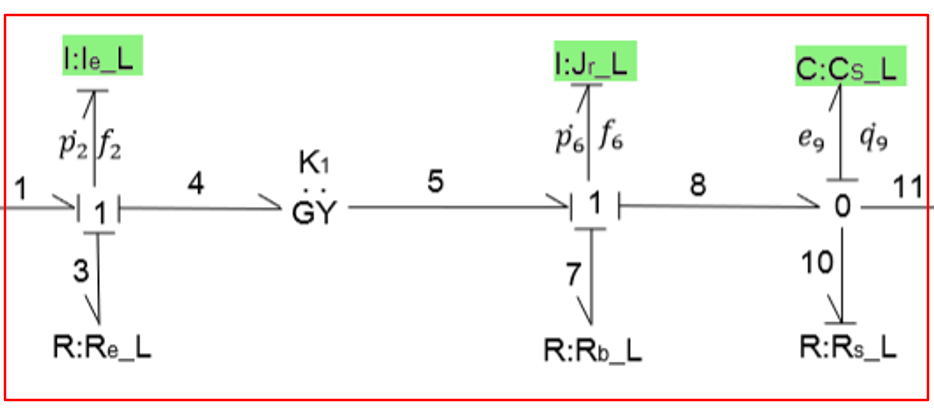
\includegraphics[width=0.5\textwidth]{fig/equation2.png}
	\caption{}\label{fig:equation2}
\end{figure}
%%%%%%%%%%%%%%%%%

对于$\dot{p} _ { 6 }$,开始列写方程,利用键合图的因果关系求出$e_6$:根据功率流方向标注,势变量$e_6$来自1结的输出,是由$e_5$,$e_7$,和$e_8$产生的,因此:
\begin{equation}\label{p6}
\dot{ p } _ { 6 } = e _ { 6 } = e _ { 5 } - e _ { 7 } - e _ { 8 },
\end{equation}
$e_5$直接与状态变量有关;$e_7$来自阻性元件$R _ { bL }$的输出;$e_8$同样直接与状态变量有关,故而有下面三式:
\begin{equation}
e _ { 5 } = k _ { 1 } f _ { 4 } = k _ { 1 } f _ { 2 } = k _ { 1 } \frac { p _ { 2 } } { I _ { eL }  },
\end{equation}

\begin{equation}
e _ { 7 } = f _ { 7 } R _ { bL }  = f _ { 6 } R _ { b L }  = \frac { p _ { 6 } } { J _ { rL }  } R _ { bL} ,
\end{equation}

\begin{equation}\label{e8}
e _ { 8 } = e _ { 9 } = \frac { q _ { 9 } } { C _ { s L}  } ,
\end{equation}

由式\ref{p6}-\ref{e8}得到状态方程2:
\begin{equation}
\dot{ p } _ { 6 } = k _ { 1 } \frac { p _ { 2 } } { I _ { e L }  } - \frac { p_ { 6 } } { J _ { rL}  } R _ { bL}  - \frac { q _ { 9 } } { C _ { sL }  }.
\end{equation}

%%%%%%%%%%%%%%%%%%%%%%%%%%%%%%%%%%%%%%%%%%%%%%%%%%%%%%%%%%%%%%%%
%%%%%%%%%%%%%%%%%%%%%%%%%%%%%%%%%%%%%%%%%%%%%%%%%%%%%%%%%%%%%%%%
%%%%%%%%%%%%%%%%%%%%%%%%%%%%%%%%%%%%%%%%%%%%%%%%%%%%%%%%%%%%%%%%
\item {电机输出轴机械特性状态变量$\dot{ q_9 }$}
%%%%%%%%%%%%%%%%%
\begin{figure*}[h]
	\centering
	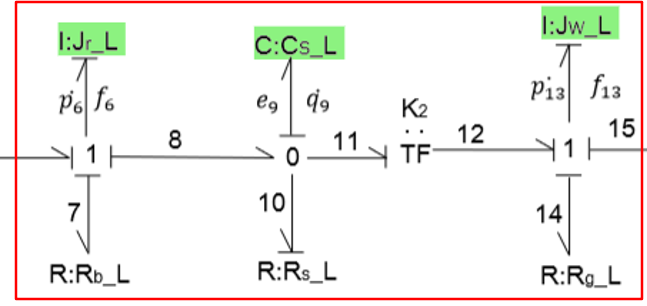
\includegraphics[width=0.5\textwidth]{fig/equation3.png}
	\caption{}\label{fig:equation3}
\end{figure*}
%%%%%%%%%%%%%%%%%
对于$\dot{q} _ { 9 }$,开始列写方程,通过使用因果关系对$f_9$路径进行跟踪,流变量$f_9$是对$C_{sL}$的输入,从0结出来的输出,此输出由因果输入$f _ { 8 }$, $ f _ { 10 }$, $  f _ { 11 }$产生,因此:
\begin{equation}\label{q9}
\dot{ q }_{ 9 } = f _ { 9 } = f _ { 8 } - f _ { 10 } - f _ { 11 },
\end{equation}
$f_8$直接与状态变量有关;$f_{10}$来自阻性元件$R _ { sL }$的输出;$f_{11}$同样直接与状态变量有关,故而有下面三式:
\begin{equation}
f _ { 8 } = f _ { 6 } = \frac { p _ { 6 } } { J _ { r L } },
\end{equation}

\begin{equation}
f _ { 10 } = \frac { e _ { 10 } } { R _ { sL}  } = \frac { e _ { 9 } } { R _ { sL }  } = \frac { q _ { 9 } } { C _ { s L}  R _ { s  L } } ,
\end{equation}

\begin{equation}\label{f11}
f _ { 11 } = \frac { f _ { 12 } } { k _ { 2 } } = \frac { f _ { 13 } } { k _ { 2 } } = \frac { p _ { 13 } } { J _ { wL}  k _ { 2 } },
\end{equation}
由式\ref{q9}-\ref{f11}得到状态方程3:
\begin{equation}
\dot{ q } _ { 9 } = \frac { p _ { 6 } } { J _ { rL } } - \frac { q _ { 9 } } { C _ { sL }  R _ { s L}  } - \frac { p _ { 13 } } { J _ { w L }  k _ { 2 } }.
\end{equation}

%%%%%%%%%%%%%%%%%%%%%%%%%%%%%%%%%%%%%%%%%%%%%%%%%%%%%%%%%%%%%%%%
%%%%%%%%%%%%%%%%%%%%%%%%%%%%%%%%%%%%%%%%%%%%%%%%%%%%%%%%%%%%%%%%
%%%%%%%%%%%%%%%%%%%%%%%%%%%%%%%%%%%%%%%%%%%%%%%%%%%%%%%%%%%%%%%%
\item{后轮机械特性状态变量$\dot{ p}_{13} $}
%%%%%%%%%%%%%%%%%
\begin{figure}[H]
	\centering
	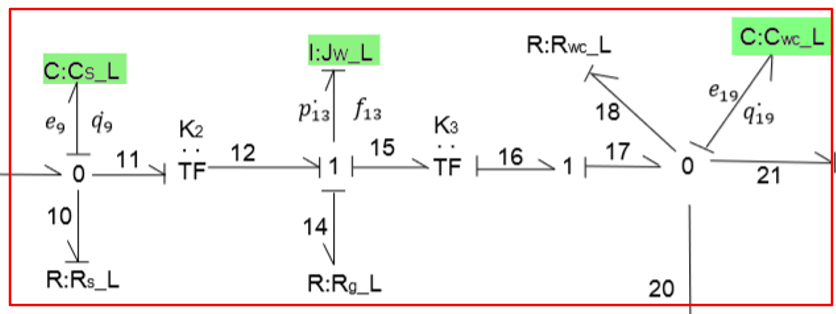
\includegraphics[width=0.5\textwidth]{fig/equation4.png}
	\caption{}\label{fig:equation4}
\end{figure}
%%%%%%%%%%%%%%%%%
对于$\dot{p} _ { 13 }$,开始列写方程,利用键合图的因果关系求出$e_{13}$:根据功率流方向标注,势变量$e_{13}$来自1结的输出,是由$e_{12}$,$e_{14}$,和$e_{15}$产生的,因此:
\begin{equation}\label{p13}
\dot{ p } _ { 13 } = e _ { 12 } - e _ { 14 } - e _ { 15 },
\end{equation}
$e_{12}$直接与状态变量有关;$e_{14}$来自阻性元件$R _ { gL }$的输出;$e_{15}$同样直接与状态变量有关,故而有下面三式:
\begin{equation}
e _ { 12 } = \frac { e _ { 11 } } { k _ { 2 } } = \frac { e _ { 9 } } { k _ { 2 } } = \frac { q _ { 9 } } { C _ { sL  } k _ { 2 } },
\end{equation}

\begin{equation}
e _ { 14 } = f _ { 14 } R _ { gL}  = f _ { 13 } R _ { gL}  = \frac { p _ { 13 } } { J _ { wL}  } R _ { gL } ,
\end{equation}

\begin{equation}\label{e15}
e _ { 15 } = e _ { 16 } k _ { 3 } = e _ { 17 } k _ { 3 } = e _ { 19 } k _ { 3 } = \frac { q _ { 19 } } { C _ { w cL }  } k _ { 3 } ,
\end{equation}
由式\ref{p13}-\ref{e15}得到状态方程4:
\begin{equation}
\dot{ p }_ { 13 } = \frac { q _ { 9 } } { C _ { sL}  k _ { 2 } } - \frac { p _ { 13 } } { J _ { wL}  } R _ { gL }  - \frac { q _ { 19 } } { C _ { w cL}  } k _ { 3 }.
\end{equation}

%%%%%%%%%%%%%%%%%%%%%%%%%%%%%%%%%%%%%%%%%%%%%%%%%%%%%%%%%%%%%%%%
%%%%%%%%%%%%%%%%%%%%%%%%%%%%%%%%%%%%%%%%%%%%%%%%%%%%%%%%%%%%%%%%
%%%%%%%%%%%%%%%%%%%%%%%%%%%%%%%%%%%%%%%%%%%%%%%%%%%%%%%%%%%%%%%%
\item{轮辐机械特性状态变量$\dot{ q}_{19}$}
%%%%%%%%%%%%%%%%%
\begin{figure*}[h]
	\centering
	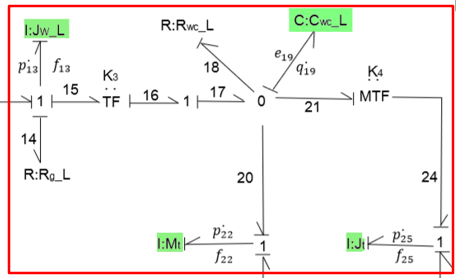
\includegraphics[width=0.5\textwidth]{fig/equation5.png}
	\caption{}\label{fig:equation5}
\end{figure*}
%%%%%%%%%%%%%%%%%
对于$\dot{q} _ { 19 }$,开始列写方程,通过使用因果关系对$f_{19}$路径进行跟踪,流变量$f_{19}$是对$C_{wcL}$的输入,从0结出来的输出,此输出由因果输入$f _ { 17 }$, $f _ { 18 }$, $ f _ { 20 }$, $  f _ { 21 }$产生,因此:
\begin{equation}\label{q19}
\dot { q } _ { 19 } = f _ { 17 } - f _ { 18 } - f _ { 20 } - f _ { 21 },
\end{equation}
$f_{17}$直接与状态变量有关;$f_{18}$来自阻性元件$R _ { wcL }$的输出;$f_{20}$和$f_{21}$同样直接与状态变量有关,故而有下面四式:
\begin{equation}
f _ { 17 } = f _ { 16 } = f _ { 15 } k _ { 3 } = f _ { 13 } k _ { 3 } = \frac { p _ { 13 } } { J _ { w L} } k _ { 3 },
\end{equation}

\begin{equation}
f _ { 18 } = \frac { e _ { 18 } } { R _ { w c L}  } = \frac { e _ { 19 } } { R _ { w cL  } } = \frac { q _ { 19 } } { C _ { w c  L} R _ { w c L } },
\end{equation}

\begin{equation}
f _ { 20 } = f _ { 22 } = \frac { p _ { 22 } } { M _ { t } },
\end{equation}

\begin{equation}\label{f21}
f _ { 21 } = \frac { f _ { 24 } } { k _ { 4 } } = \frac { f _ { 25 } } { k _ { 4 } } = \frac { p _ { 25 } } { J _ { t } k _ { 4 } },
\end{equation}
由式\ref{q19}-\ref{f21}得到状态方程5:
\begin{equation}
\dot { q } _ { 19 } = \frac { p _ { 13 } } { J _ { w L }  } k _ { 3 } - \frac { q _ { 19 } } { C _ { w c L }  R _ { w c L }  } - \frac { p _ { 22 } } { M _ { t } } - \frac { p _ { 25 } } { J _ { t } k _ { 4 } }.
\end{equation}

%%%%%%%%%%%%%%%%%%%%%%%%%%%%%%%%%%%%%%%%%%%%%%%%%%%%%%%%%%%%%%%%
%%%%%%%%%%%%%%%%%%%%%%%%%%%%%%%%%%%%%%%%%%%%%%%%%%%%%%%%%%%%%%%%
%%%%%%%%%%%%%%%%%%%%%%%%%%%%%%%%%%%%%%%%%%%%%%%%%%%%%%%%%%%%%%%%
\item {质心处状态分析(质量)状态变量$\dot{ p}_{22} $}
%%%%%%%%%%%%%%%%%
\begin{figure}[H]
	\centering
	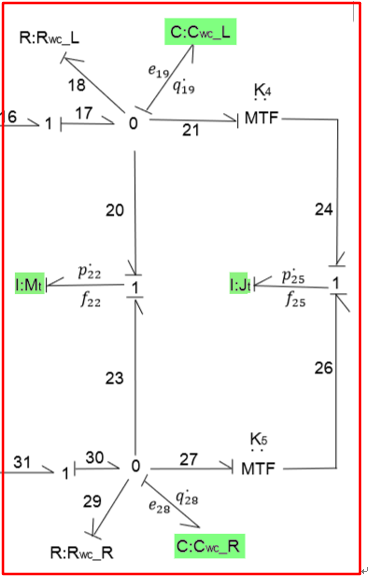
\includegraphics[width=0.25\textwidth]{fig/equation6.png}
	\caption{}\label{fig:equation6}
\end{figure}
%%%%%%%%%%%%%%%%%
对于$\dot{p} _ { 22 }$,开始列写方程,利用键合图的因果关系求出$e_{22}$:根据功率流方向标注,势变量$e_{22}$来自1结的输出,是由$e_{20}$和$e_{23}$产生的,因此:
\begin{equation}\label{p22}
\dot{ p }  _ { 22 } = e _ { 22 } = e _ { 20 } + e _ { 23 },
\end{equation}
$e_{20}$与$e_{23}$均直接与状态变量有关,故而有下面两式:
\begin{equation}
e _ { 20 } = e _ { 19 } = \frac { q _ { 19 } } { C _ { w cL }  },
\end{equation}

\begin{equation}\label{e23}
e _ { 23 } = e _ { 28 } = \frac { q _ { 28 } } { C _ { w c R }  },
\end{equation}
由式\ref{p22}-\ref{e23}得到状态方程6:
\begin{equation}
\dot{ p } _ { 22 } = \frac { q _ { 19 } } { C _ { w c L } } + \frac { q _ { 28 } } { C _ { w c R  } }.
\end{equation}

%%%%%%%%%%%%%%%%%%%%%%%%%%%%%%%%%%%%%%%%%%%%%%%%%%%%%%%%%%%%%%%%
%%%%%%%%%%%%%%%%%%%%%%%%%%%%%%%%%%%%%%%%%%%%%%%%%%%%%%%%%%%%%%%%
%%%%%%%%%%%%%%%%%%%%%%%%%%%%%%%%%%%%%%%%%%%%%%%%%%%%%%%%%%%%%%%%
\item {质心处状态分析(转动惯量)状态变量$\dot{ p}_{25} $}
%%%%%%%%%%%%%%%%%
\begin{figure}[H]
	\centering
	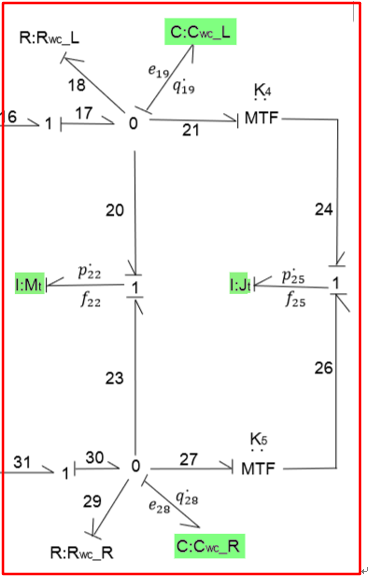
\includegraphics[width=0.25\textwidth]{fig/equation6.png}
	\caption{}\label{fig:equation6}
\end{figure}
%%%%%%%%%%%%%%%%%
对于$\dot{p} _ { 25 }$,开始列写方程,利用键合图的因果关系求出$e_{25}$:根据功率流方向标注,势变量$e_{22}$来自1结的输出,是由$e_{24}$和$e_{26}$产生的,因此:
\begin{equation}\label{p25}
\dot{ p } _ { 25 } = e _ { 24 } + e _ { 26 },
\end{equation}
$e_{24}$与$e_{26}$均直接与状态变量有关,故而有下面两式:
\begin{equation}
e _ { 24 } = \frac { e _ { 21 } } { k _ { 4 } } = \frac { e _ { 19 } } { k _ { 4 } } = \frac { q _ { 19 } } { C _ { w cL}  k _ { 4 } },
\end{equation}

\begin{equation}\label{e26}
e _ { 26 } = \frac { e _ { 27 } } { k _ { 5 } } = \frac { e _ { 28 } } { k _ { 5 } } = \frac { q _ { 28 } } { C _ { w c L }  k _ { 5 } },
\end{equation}
由式\ref{p25}-\ref{e26}得到状态方程7:
\begin{equation}
\dot{ p } _ { 25 } = \frac { q _ { 19 } } { C _ { w c L}  k _ { 4 } } + \frac { q _ { 28 } } { C _ { w cL }  k _ { 5 } }.
\end{equation}
%%%%%%%%%%%%%%%%%%%%%%%%%%%%%%%%%%%%%%%%%%%%%%%%%%%%%%%%%%%%%%%%
%%%%%%%%%%%%%%%%%%%%%%%%%%%%%%%%%%%%%%%%%%%%%%%%%%%%%%%%%%%%%%%%
%%%%%%%%%%%%%%%%%%%%%%%%%%%%%%%%%%%%%%%%%%%%%%%%%%%%%%%%%%%%%%%%
\item {根据对称性得到剩余状态方程}
根据对称性,另外五个状态方程见\ref{q28}-\ref{p44}:
\begin{equation}\label{q28}
\dot{ q}  _ { 28 } = \frac { p _ { 33 } } { J _ { w R }  } k _ { 6 } - \frac { q _ { 28 } } { C _ { w cR }  R _ { w c R } } - \frac { p _ { 22 } } { M _ { t } } - \frac { p _ { 25 } } { J _ { t } k _ { 5 } }.
\end{equation}

\begin{equation}
\dot{ p } _ { 33 } = \frac { q _ { 37 } } { C _ { s R }  k _ { 7 } } - \frac { p _ { 33 } } { J _ { wR }  } R _ { gR }  - \frac { q _ { 28 } } { C _ { w cR }  } k _ { 6 }
\end{equation}

\begin{equation}
\dot{q} _ { 37 } = \frac { p _ { 40 } } { J _ { r R } } - \frac { q _ { 37 } } { C _ { sR }  R _ { sR}  } - \frac { p _ { 33 } } { J _ { w R}  k _ { 7 } }
\end{equation}

\begin{equation}
\dot{ p } _ { 40 } = k _ { 8 } \frac { p _ { 44 } } { I _ { e R}  } - \frac { p _ { 40 } } { J _ { r R }  } R _ { b R }  - \frac { q _ { 37 } } { C _ { s R } }
\end{equation}

\begin{equation}\label{p44}
\dot{ p } _ { 44 } = V _ {R}  - \frac { p _ { 44 } } { I _ { e R} } R _ { e R }  - k _ { 8 } \frac { p _ { 40 } } { J _ { r R  } }
\end{equation}
\subsection{总体状态空间矩阵}

\end{enumerate}

\subsubsection{状态空间矩阵导出}

下列公式显示了MDW的状态空间表示,其中$ x_2$,$u_2$和$y_2$分别是系统状态,输入和输出:

\begin{equation}\label{2_dot_x2}
\dot{x}_2 =[\mathbf{A}_2] x_2+[\mathbf{B}_2] u_2,
\end{equation}

\begin{equation}\label{2_y2}
y_2 =[\mathbf{C}_2] x_2.
\end{equation}

由上述12个状态空间方程,具体表示成:
\begin{small}
	\begin{equation}\label{1_matrix1}
	\begin{aligned}
	\left[ 
	\begin{array}
	{l}{e_{2}} \\ {e_{6}}\\ {f_{9}} \\ {e_{13}}\\ {f_{19}} \\ {e_{22}} \\ {e_{25}} \\ {f_{28}} \\ {e_{33}} \\ {f_{37}} \\ {e_{40}}\\ {e_{44}}
	\end{array}
	\right] 
	=
	\left[ 
	\begin{array}
	{c}{\dot{p}_{2}} \\ {\dot{p}_{6}} \\ {\dot{q}_{9}}\\ {\dot{p}_{13}}\\ {\dot{q}_{19}}\\ {\dot{p}_{22}} \\ {\dot{p}_{25}}\\ {\dot{q}_{28}}\\ {\dot{p}_{33}}  \\ {\dot{q}_{37}} \\ {\dot{p}_{40}} \\ {\dot{p}_{44}} 
	\end{array}
	\right]
	=
    &\left[ 
	\begin{array}{cccccccccccc}
	{- \frac { R _ { eL}} { I _ { eL}  } } &  \frac {k _ { 1 }} { J _ { rL} }  &0& 0 & 0 & 0 & 0 & 0 & 0 & 0 & 0 & 0 \\
	\frac {k _ { 1 }} { I _ { e L }  } & - \frac {  R _ { bL} } { J _ { rL}  } &  - \frac { 1} { C _ { sL }  } & 0 & 0 & 0 & 0 & 0& 0 & 0 & 0 & 0  \\ 
	0  & \frac {1} { J _ { rL } }  & - \frac { 1} { C _ { sL }  R _ { s L}  } & - \frac { 1 } { J _ { w L }  k _ { 2 } }&0 & 0 & 0 & 0 & 0 & 0 & 0 & 0  \\ 
	0 & 0 & \frac{1}{C_{wc L}k_2} & - \frac {  R _ { gL }} { J _ { wL}  } & - \frac {k _ { 3 } } { C _ { w cL}  }  & 0 & 0 & 0 & 0 & 0 & 0 & 0   \\ 
	0 & 0 & 0 & \frac {  k _ { 3 }  } { J _ { w L }  } & - \frac {1} { C _ { w c L } R _ { w c L }   } &- \frac { 1 } { M _ { t } }  &  - \frac { 1} { J _ { t } k _ { 4 } } & 0 & 0 & 0 & 0 & 0  \\ 
	0 & 0 & 0 & 0 &  \frac{1}{ C_{wc L}} & 0& 0 & - \frac{1}{C_{wc R}} & 0 & 0 & 0 & 0  \\ 
	0 & 0 & 0 & 0 &\frac { 1 } { C _ { w c L}  k _ { 4 } } & 0 & 0 & \frac { 1 } { C _ { w cR }  k _ { 5 } }& 0 & 0 & 0 & 0  \\ 
	0 & 0 & 0 & 0 & 0 & - \frac {1 } { M _ { t } } & - \frac { 1 } { J _ { t } k _ { 5 } } & - \frac {1 } { C _ { w cR }  R _ { w c R } } &  \frac {  k _ { 6 }  } { J _ { w R }  } & 0 & 0 & 0 \\
	0 & 0 & 0 & 0 & 0 & 0& 0 & - \frac { k _ { 6 }} { C _ { w cR }  } & - \frac {R _ { gR }  } { J _ { wR }  }  & \frac { k _ { 7 } } { C _ { s R }  } & 0 & 0 \\
	0 & 0 & 0 & 0 & 0 & 0& 0 & 0 & - \frac {1} { J _ { w R}  k _ { 7 } } & - \frac { 1} { C _ { sR }  R _ { sR}  }  & \frac {1 } { J _ { r R } }  & 0 \\
	0 & 0 & 0 & 0 & 0 & 0& 0 & 0 & 0 &  - \frac { 1} { C _ { s R } } &  - \frac { R _ { b R } } { J _ { r R }  }  & \frac {k _ { 8 }  } { I _ { e R}  }  \\
	0 & 0 & 0 & 0 & 0 & 0& 0 & 0 & 0 & 0 &  \frac { - k _ { 8 } } { J _ { r R  } } &- \frac {R _ { e R } } { I _ { e R} } 
	
	\end{array}
    \right]
    \\    
	&\left[
	\begin{array}{c}
	{p_{2}} \\ {{p}_{6}} \\ {{q}_{9}}\\ {{p}_{13}}\\ {{q}_{19}}\\ {{p}_{22}} \\ {{p}_{25}}\\ {{q}_{28}}\\ {{p}_{33}}  \\ {{q}_{37}} \\ {{p}_{40}} \\ {{p}_{44}} 
	\end{array}
	\right]
	+
	\left[ 
	\begin{array}{ll}
	{1} & {0} \\ {0} & {0}\\ {0} & {0} \\ {0} & {0} \\ {0} & {0} \\ {0} & {0}  \\ {0} & {0} \\ {0} & {0} \\ {0} & {0} \\ {0} & {0} \\ {0} & {0} \\ {0} & {1}
	\end{array}
	\right]
	\left[ 
	\begin{array}{l}
	{V_{L}} \\ {V_{R}}
	\end{array}
	\right]
	\end{aligned}
	\end{equation}
\end{small}
则输出矩阵则表示为:

\begin{equation}\label{1_matrix2}
\left[
\begin{array}{c}{i_{L}} \\ {\tau_{L}}  \\ {\omega_{mL}}\\ {\omega_{wL}} \\ {V_{C G}} \\ {\theta_{C G}}\\ {\omega_{mR}}\\ {\omega_{wR}}\\{\tau_{R}} \\ {i_{R}}
\end{array}
\right]
=
\left[
\begin{array}{c}{i_{2}} \\ {e_{6}} \\ {f_{8}} \\ {f_{13}}\\ {f_{22}} \\ {f_{25}}\\ {f_{33}}\\ {f_{39}}\\ {e_{40}}\\ {i_{44}}\end{array}
\right]
=
\left[ \begin{array}{cccccccc}
{\frac{1}{I_{e L}}} & {0} & {0} & {0} & {0} & {0} & {0} & {0} \\
 {\frac{k_1}{J_{r L}}} & 0 & {0} & {0}& {0} & {0} & {0} & {0} \\  
0 & {\frac{1}{J_{r L}}} &0 & {0}& {0} & {0} & {0} & {0}  \\ 
 {0} & {0} & {\frac{1}{J_{w L}}} & 0& {0} & {0} & {0} & {0} \\
 {0} & {0} & {0} & {\frac{1}{M_{t}}}& {0} & {0} & {0} & {0} \\
 {0} & {0} & {0} & {0} &{\frac{1}{J_{t}}}& {0} & {0} & {0}\\
 {0} & {0} & {0} &0& {0} & {\frac{1}{J_{wR}}} & {0} & {0} \\
  {0} & {0} & {0} &0& {0} & 0 & {\frac{1}{J_{rR}}} & {0} \\
    {0} & {0} & {0} &0& {0} & 0 & 0& {\frac{k_8}{J_{rR}}}  \\
     {0} & {0} & {0} &0& {0} & 0 & 0& {\frac{1}{I_{eR}}} 
\end{array}\right] 
\left[ \begin{array}{c}
{p_{2}} \\ {p_{6}} \\ {p_{13}} \\ {p_{22}}\\{p_{25}} \\ {p_{33}} \\ {p_{40}} \\ {p_{44}}
\end{array}\right].
\end{equation}


	\clearpage
\section{实验阶段}

\subsection{实验参数设定}

表 \ref{tab:param} 列出本模型的相关参数及其数学标记。本报告中表示左右参数则分别以 $ \_L $ 和 $ \_R $表示。参数表主要分为分为整体系统参数,手推轮椅主体,机电驱动模块以及手推控制输入部分的参数四个部分。如下所示(见下页):

\begin{table}[H]
	\footnotesize
	\caption{系统主要参数及其数学标记}\label{tab:param}
	\begin{longtable}{l|l|l}
		\toprule
		\textbf{数学标记} & \textbf{系统参数} & \textbf{设计值}\\
		\midrule
		\endhead
		\multicolumn{3}{l}{\textbf{系统整体参数}} \\ % {占用行数} {文字居左中右} {内容}
		\midrule
		$ V_{\rm{CG}} $ & 质心速度 & \\
		$ w_{\rm{CG}} $ & 质心转速 & \\
		$ P_{\rm{CG}} $ & 系统动量变化率 & \\
		$ P_{\theta} $ & 系统角动量变化率 & \\
		\midrule
		\multicolumn{3}{l}{\textbf{手推轮椅主体}} \\
		\midrule
		SE:$\tau$ & 后轮推进扭矩($ \mathrm{N} \cdot \mathrm{m} $) & 12 \\
		$ J w $ & 后轮转动惯量($ \mathrm{kg} \cdot \mathrm{m}^2 $) & 0.005 \\
		$ M_t $ & 系统质量 & \\
		$ J t $ & 系统转动惯量 & \\
		$ R_g $ & 轮胎与地面摩擦系数 & \\
		$ C_w $ & 轮辐弹性系数 & \\
		$ R_w $ & 轮辐阻尼 & \\
		$ r $ & 后轮半径 & \\
		$ L_w $ & 轮椅宽度 & \\
		$ R_{wc} $ & 联轴器阻尼系数 & \\
		$ C_{wc} $ & 联轴器弹性系数 & \\
		\midrule
		\multicolumn{3}{l}{\textbf{机电驱动模块}} \\
		\midrule
		$ I_e $ & 电机电感 & \\
		$ R_e $ & 电机内阻 & \\
		$ J_r $ & 转子转动惯量 & \\
		$ R_b $ & 电机轴承阻尼 & \\
		$ M_d $ & 机电驱动模块质量 & \\
		$ J_d $ & 机电驱动模块转动惯量 & \\
		$ L_d $ & 模块宽度 & \\
		$ C_s $ & 电机输出转矩 & \\
		$ R_s $ & 电机输出轴阻尼 & \\
		$ k_1 $ & 电机扭矩系数 & \\ % 简化了k8
		$ k_2 $ & 齿轮系数比 & \\ % 简化了k7
		$ k_3 $ & 电动车轮半径 & \\ % 简化了k6
		Se:L & 输入控制电压\\
		\midrule
		\multicolumn{3}{l}{\textbf{手推控制输入部分}}\\
		\midrule
		$ J $ & 手动轮转动惯量 & \\
		$ k_4 $ & 手动轮半径 & \\ % 简化了k10
		\bottomrule
	\end{longtable}
\end{table}
	\clearpage
\section{系统总体模型}

在本文中,在将原有的机械主体部分和电驱动模块连接在一起,我们便得到了总体的键合图,从而验证最初的系统分析的合理性,机械主题部分和电驱动模块的
通过机械连接后,便生成了总体键合图,如下图~\ref{fig:overall}所示。

%%%%%%%%%%%%%%%%%
\begin{figure*}[!h]
	\centering
	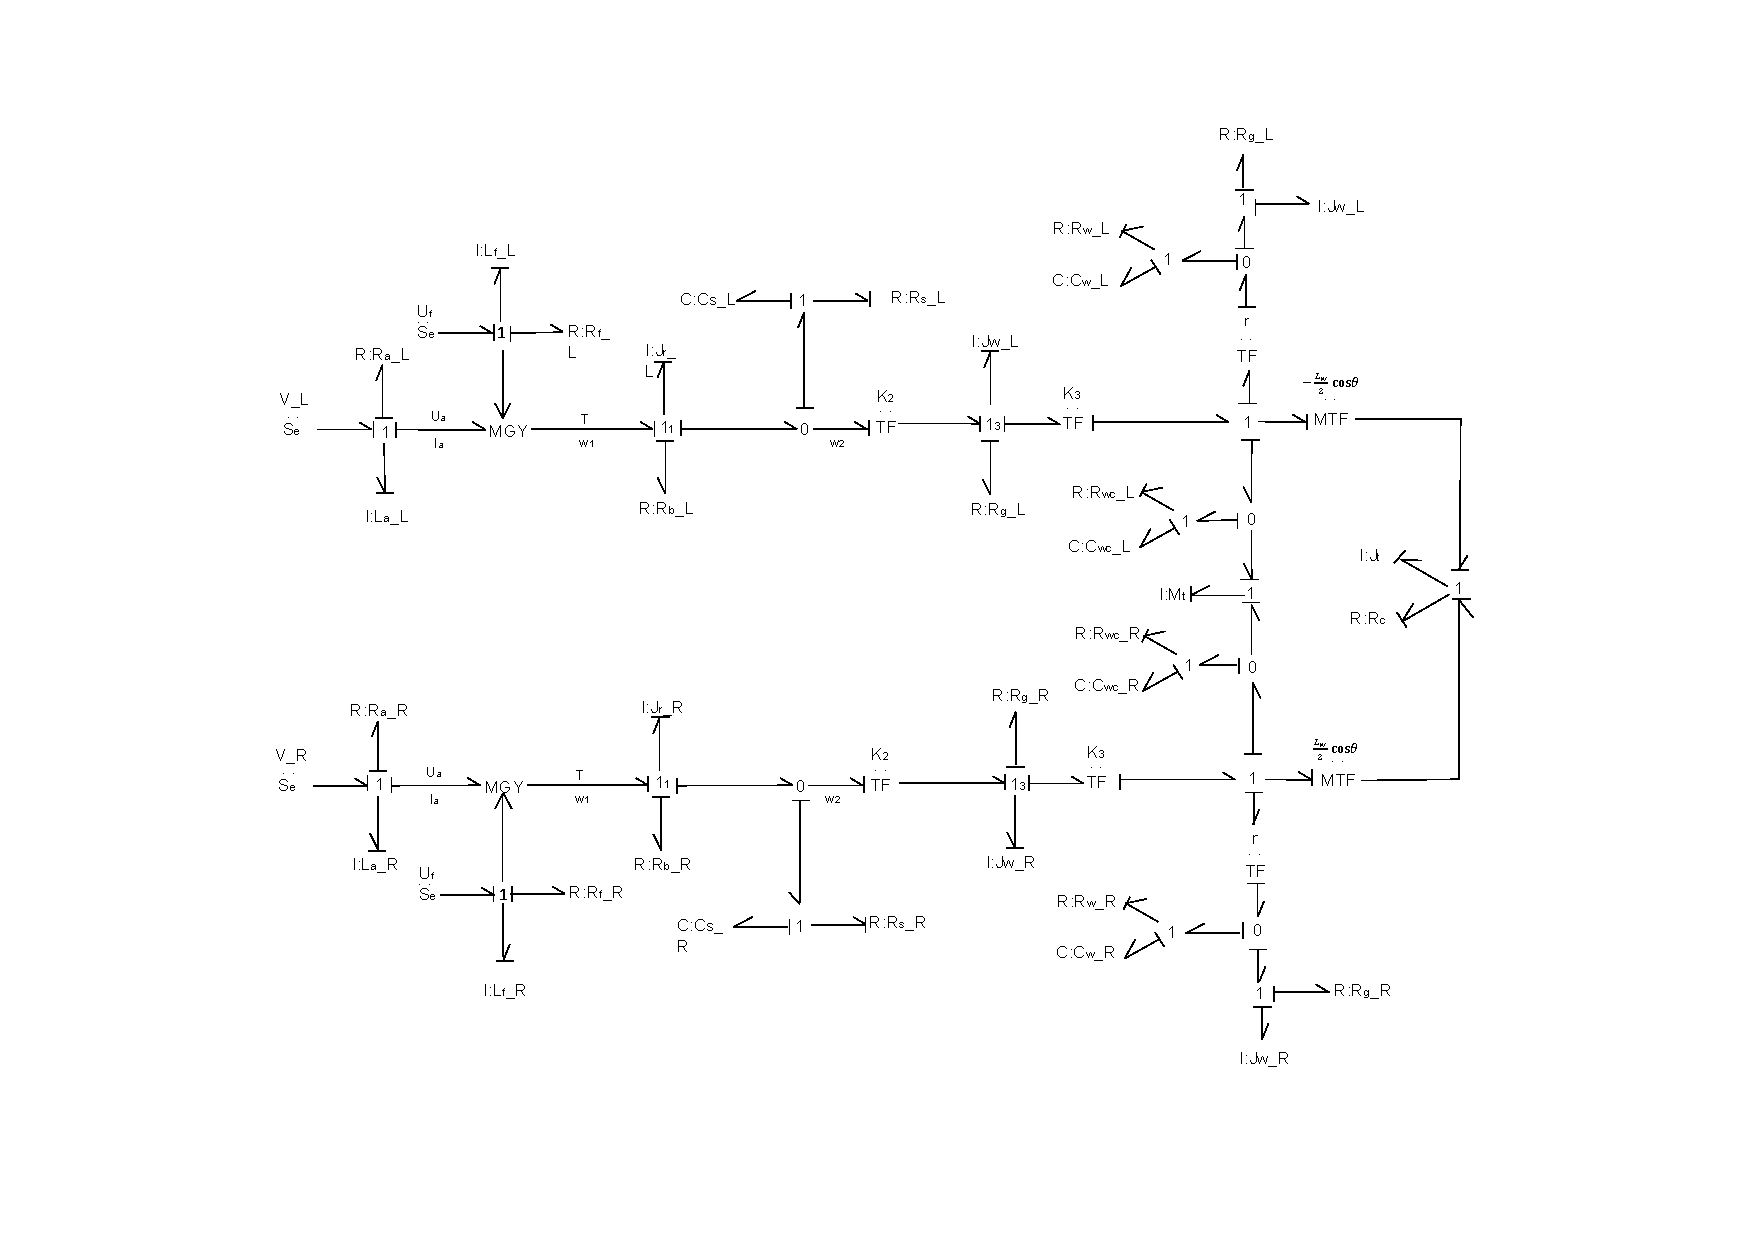
\includegraphics[width=1.25\textwidth,angle=90]{fig/overall.pdf}
	\caption{总体键合图。}\label{fig:overall}
\end{figure*}
%%%%%%%%%%%%%%%%%
	\newpage
\addcontentsline{toc}{section}{参考文献}
\begin{thebibliography}{0}
	
	\bibitem{System_Dynamics_Modeling}
	D. C. Karnopp, D. L. Margolis, and R. C. Rosenberg, System Dynamics Modeling and Simulation of Mechatronic Systems (Fourth Edition) [M]. New York: Wiley, 2012.
		
	\bibitem{System_Dynamics_Modeling_cn}
	D. C. Karnopp, D. L. Margolis, and R. C. Rosenberg, 黎明安(译), 系统动力学——机电系统的建模与仿真 [M]. 国防工业出版社, 2012.
	
	\bibitem{Simulation1}
	Klee H , Allen R . Simulation of dynamic systems with MATLAB and Simulink. 2nd ed[M]// Simulation of Dynamic Systems with MATLAB and Simulink. CRC Press, Inc. 2007.
	
	\bibitem{Simulation2}
	Wouwer A V . Simulation Of ODE/PDE Models With MATLAB®, OCTAVE And SCILAB[J]. Annals of the Rheumatic Diseases, 2014, 71(Suppl 3):646-646.
	
	\bibitem{wheelchairs_review}
	Leaman, Jesse, and Hung Manh La. A comprehensive review of smart wheelchairs: past, present, and future [J]. IEEE Transactions on Human-Machine Systems 47.4 2017: 486-499.
	
	\bibitem{Bond_graph_methodology}
	Borutzky, W. Bond graph methodology, development and analysis of multidisciplinary dynamic system models (1st ed.) [M]. Berlin: Springer. 2010
	
	\bibitem{Bond_graph_modelling}
	Borutzky, Wolfgang. Bond graph modelling of engineering systems  [M]. Vol. 103. New York: Springer, 2011.
	
	\bibitem{Ayala2015ROBIO}
	Ayala, Gerardo, Rui Loureiro, and Rochdi Merzouki. Multi-domain model of steering system for an omnidirectional mobile robot  [C]. 2015 IEEE International Conference on Robotics and Biomimetics (ROBIO). IEEE, 2015.
	
	\bibitem{Sahoo2016RCTFC}
	Sahoo, Saumya Ranjan, and Shital S. Chiddarwar. Dynamic modelling of four wheel skid mobile robot by unified bond graph approach [C]. 2016 International Conference on Robotics: Current Trends and Future Challenges (RCTFC). IEEE, 2016.
	
	\bibitem{Jahanbin2016JBSMSE}
	Jahanbin, Zahra, et al. Multi-body simulation of a flapping-wing robot using an efficient dynamical model [J]. Journal of the Brazilian Society of Mechanical Sciences and Engineering 38.1 (2016): 133-149.
	
	\bibitem{Proceedings1}
	Fakri, A., Vilakazi, J. P. Modular driven wheelchair bond graph modelling [C]. The European Modeling \& Simulation Symposium, I3M2010 MultiConference, 2010, Fes, Morocco.
	
	\bibitem{Proceedings2}
	Fakri, A., Vilakazi, J. P. Wheelchair and electric drive add-on a whole bond graph modelling [C]. Proceedings of the 2014 11th International Conference on Bond graph Modeling and Simulation (ICBGM’14). SummerSim 2014 Multiconference July 6–10 2014, Monterey, CA, USA. ISBN: 978-1-63266-700-7, Vol. 46 \#8, Collection:Simulation Series, 206-210, 222 pp. 113.
	
\end{thebibliography}

\end{document}
